% Options for packages loaded elsewhere
\PassOptionsToPackage{unicode}{hyperref}
\PassOptionsToPackage{hyphens}{url}
\PassOptionsToPackage{dvipsnames,svgnames,x11names}{xcolor}
%
\documentclass[
  10pt,
]{article}
\usepackage{amsmath,amssymb}
\usepackage{lmodern}
\usepackage{iftex}
\ifPDFTeX
  \usepackage[T1]{fontenc}
  \usepackage[utf8]{inputenc}
  \usepackage{textcomp} % provide euro and other symbols
\else % if luatex or xetex
  \usepackage{unicode-math}
  \defaultfontfeatures{Scale=MatchLowercase}
  \defaultfontfeatures[\rmfamily]{Ligatures=TeX,Scale=1}
\fi
% Use upquote if available, for straight quotes in verbatim environments
\IfFileExists{upquote.sty}{\usepackage{upquote}}{}
\IfFileExists{microtype.sty}{% use microtype if available
  \usepackage[]{microtype}
  \UseMicrotypeSet[protrusion]{basicmath} % disable protrusion for tt fonts
}{}
\makeatletter
\@ifundefined{KOMAClassName}{% if non-KOMA class
  \IfFileExists{parskip.sty}{%
    \usepackage{parskip}
  }{% else
    \setlength{\parindent}{0pt}
    \setlength{\parskip}{6pt plus 2pt minus 1pt}}
}{% if KOMA class
  \KOMAoptions{parskip=half}}
\makeatother
\usepackage{xcolor}
\usepackage[left=2cm, right=2cm, top=2cm, bottom=3cm, footskip = .5cm]{geometry}
\usepackage{longtable,booktabs,array}
\usepackage{calc} % for calculating minipage widths
% Correct order of tables after \paragraph or \subparagraph
\usepackage{etoolbox}
\makeatletter
\patchcmd\longtable{\par}{\if@noskipsec\mbox{}\fi\par}{}{}
\makeatother
% Allow footnotes in longtable head/foot
\IfFileExists{footnotehyper.sty}{\usepackage{footnotehyper}}{\usepackage{footnote}}
\makesavenoteenv{longtable}
\usepackage{graphicx}
\makeatletter
\def\maxwidth{\ifdim\Gin@nat@width>\linewidth\linewidth\else\Gin@nat@width\fi}
\def\maxheight{\ifdim\Gin@nat@height>\textheight\textheight\else\Gin@nat@height\fi}
\makeatother
% Scale images if necessary, so that they will not overflow the page
% margins by default, and it is still possible to overwrite the defaults
% using explicit options in \includegraphics[width, height, ...]{}
\setkeys{Gin}{width=\maxwidth,height=\maxheight,keepaspectratio}
% Set default figure placement to htbp
\makeatletter
\def\fps@figure{htbp}
\makeatother
\setlength{\emergencystretch}{3em} % prevent overfull lines
\providecommand{\tightlist}{%
  \setlength{\itemsep}{0pt}\setlength{\parskip}{0pt}}
\setcounter{secnumdepth}{-\maxdimen} % remove section numbering
\newlength{\cslhangindent}
\setlength{\cslhangindent}{1.5em}
\newlength{\csllabelwidth}
\setlength{\csllabelwidth}{3em}
\newlength{\cslentryspacingunit} % times entry-spacing
\setlength{\cslentryspacingunit}{\parskip}
\newenvironment{CSLReferences}[2] % #1 hanging-ident, #2 entry spacing
 {% don't indent paragraphs
  \setlength{\parindent}{0pt}
  % turn on hanging indent if param 1 is 1
  \ifodd #1
  \let\oldpar\par
  \def\par{\hangindent=\cslhangindent\oldpar}
  \fi
  % set entry spacing
  \setlength{\parskip}{#2\cslentryspacingunit}
 }%
 {}
\usepackage{calc}
\newcommand{\CSLBlock}[1]{#1\hfill\break}
\newcommand{\CSLLeftMargin}[1]{\parbox[t]{\csllabelwidth}{#1}}
\newcommand{\CSLRightInline}[1]{\parbox[t]{\linewidth - \csllabelwidth}{#1}\break}
\newcommand{\CSLIndent}[1]{\hspace{\cslhangindent}#1}
% Set up the fonts
\usepackage[urw-palatino]{mathdesign}
\usepackage[T1]{fontenc}

% Add accessibility support from http://www.richschwinn.com/accessibility
\RequirePackage{accsupp}
\RequirePackage{pdfcomment}
\newcommand{\AccTool}[2]{\BeginAccSupp{method=pdfstringdef,unicode,Alt={{#1}}}\pdftooltip{{#2}}{{#1}}\EndAccSupp{}}

% Set the language for 508
\hypersetup{
  pdftitle = {title},
  pdflang = en-US}


% Set up the headers and footers
\usepackage{graphicx}
\usepackage{fancyhdr}
\usepackage{ifthen}
%\usepackage{everypage-1x}
\usepackage{float}
%\usepackage{subfig}
%\usepackage{subcaption}

% Avoid struggling over figure and table float in Rmarkdown
\let\origfigure\figure
\let\endorigfigure\endfigure
\renewenvironment{figure}[1][2] {
    \expandafter\origfigure\expandafter[H]
} {
    \endorigfigure
}

\let\origtable\table
\let\endorigtable\endtable
\renewenvironment{table}[1][2] {
    \expandafter\origtable\expandafter[H]
} {
    \endorigtable
}

% First page has the large title and NOAA logo
\pagestyle{fancy}
\fancyhf{}
\setlength\headheight{40pt}
\fancyheadoffset[L]{0.5cm}
\cfoot{\thepage}

\fancyheadinit{%
   \ifthenelse{\value{page}=5}%
      {\fancyhead[R]{
\includegraphics[width=40pt]{images/NOAA_logo.png} \\ \textsf{\emph{February 9, 2023}}}
       \fancyhead[L]{\textsf{\LARGE DRAFT State of the Ecosystem 2024: New England}}
      }%
      {\fancyhead[R]{}
       \fancyhead[L]{\textsf{\emph{DRAFT State of the Ecosystem 2024: New England}}}
      }
}



\renewcommand{\headrulewidth}{0.4pt}
\renewcommand{\footrulewidth}{0pt}

% Make caption fonts a bit smaller
\usepackage[font={small}]{caption}


% Change section labels to san serif
\usepackage{sectsty}
\allsectionsfont{\normalfont\sffamily\bfseries}
\usepackage{multirow}
\usepackage{multicol}
\usepackage{colortbl}
\usepackage{hhline}
\usepackage{longtable}
\usepackage{float}
\usepackage{wrapfig}
\usepackage{array}
\usepackage{hyperref}
\ifLuaTeX
  \usepackage{selnolig}  % disable illegal ligatures
\fi
\IfFileExists{bookmark.sty}{\usepackage{bookmark}}{\usepackage{hyperref}}
\IfFileExists{xurl.sty}{\usepackage{xurl}}{} % add URL line breaks if available
\urlstyle{same} % disable monospaced font for URLs
\hypersetup{
  colorlinks=true,
  linkcolor={Maroon},
  filecolor={Maroon},
  citecolor={Blue},
  urlcolor={blue},
  pdfcreator={LaTeX via pandoc}}

\author{}
\date{\vspace{-2.5em}}

\begin{document}

\setcounter{page}{5}
\thispagestyle{fancy}

\hypertarget{introduction}{%
\section{Introduction}\label{introduction}}

\hypertarget{about-this-report}{%
\subsection{About This Report}\label{about-this-report}}

This report is for the New England Fishery Management Council (NEFMC). The purpose of this report is to synthesize ecosystem information to allow the NEFMC to better meet fishery management objectives. The major messages of the report are summarized on pages 1, 2, and 3, and synthesis themes are illustrated on page 4. Information in this report is organized into two sections; \protect\hyperlink{performance-relative-to-fishery-management-objectives}{performance measured against ecosystem-level management objectives} (Table \ref{tab:management-objectives}), and potential \protect\hyperlink{risks-to-meeting-fishery-management-objectives}{risks to meeting fishery management objectives} (\protect\hyperlink{climate-and-ecosystem-productivity}{climate change} and \protect\hyperlink{other-ocean-uses-offshore-wind}{other ocean uses}).

\hypertarget{report-structure}{%
\subsection{Report structure}\label{report-structure}}

The two main sections contain subsections for each management objective or potential risk. Within each subsection, we first review indicator trends, and the status of the most recent data year relative to a threshold (if available) or relative to the long-term average. Second, we synthesize results of other indicators and information to outline potential implications for management (i.e., connecting indicator(s) status to management and why an indicator(s) is important). For example, if there are multiple drivers related to an indicator trend, which drivers may be more or less supported by current information, and which, if any, can be affected by management action(s)? Similarly, which risk indicators warrant continued monitoring to evaluate whether regime shifts or ecosystem reorganization are likely? We emphasize that these implications are intended to represent testable hypotheses at present, rather than ``answers,'' because the science behind these indicators and syntheses continues to develop.

A glossary of terms\footnote{\url{https://noaa-edab.github.io/tech-doc/glossary.html}}, detailed technical methods documentation\footnote{\url{https://NOAA-EDAB.github.io/tech-doc}} and indicator data\footnote{\url{https://github.com/NOAA-EDAB/ecodata}}, and detailed indicator descriptions\footnote{\url{https://noaa-edab.github.io/catalog/index.html}} are available online. The details of standard figure formatting (Fig. \ref{fig:docformat}a), categorization of fish and invertebrate species into feeding groups (Table \ref{tab:species-groupings}), and definitions of ecological production units (EPUs, including Georges Bank, GB, and the Gulf of Maine, GOM; Fig. \ref{fig:docformat}b) are provided at the end of the document.

\providecommand{\docline}[3]{\noalign{\global\setlength{\arrayrulewidth}{#1}}\arrayrulecolor[HTML]{#2}\cline{#3}}

\setlength{\tabcolsep}{0pt}

\renewcommand*{\arraystretch}{1}

\begin{longtable}[c]{|p{1.42in}|p{4.09in}}

\caption{\textcolor[HTML]{000000}{\fontsize{9}{11}\selectfont{Example\ ecosystem-scale\ fishery\ management\ objectives\ for\ the\ New\ England\ region}}}\label{tab:management-objectives}\\

\hhline{>{\arrayrulecolor[HTML]{666666}\global\arrayrulewidth=2pt}->{\arrayrulecolor[HTML]{666666}\global\arrayrulewidth=2pt}-}

\multicolumn{1}{!{\color[HTML]{000000}\vrule width 0pt}>{\raggedright}p{\dimexpr 1.42in+0\tabcolsep+0\arrayrulewidth}}{\textcolor[HTML]{000000}{\fontsize{9}{9}\selectfont{Objective\ categories}}} & \multicolumn{1}{!{\color[HTML]{000000}\vrule width 0pt}>{\raggedright}p{\dimexpr 4.09in+0\tabcolsep+0\arrayrulewidth}!{\color[HTML]{000000}\vrule width 0pt}}{\textcolor[HTML]{000000}{\fontsize{9}{9}\selectfont{Indicators\ reported}}} \\

\hhline{>{\arrayrulecolor[HTML]{666666}\global\arrayrulewidth=2pt}->{\arrayrulecolor[HTML]{666666}\global\arrayrulewidth=2pt}-}\endhead



\multicolumn{2}{!{\color[HTML]{000000}\vrule width 0pt}>{\raggedright}p{\dimexpr 5.51in+2\tabcolsep+1\arrayrulewidth}!{\color[HTML]{000000}\vrule width 0pt}}{\textcolor[HTML]{000000}{\fontsize{9}{9}\selectfont{\textbf{Provisioning\ and\ Cultural\ Services}}}} \\





\multicolumn{1}{!{\color[HTML]{000000}\vrule width 0pt}>{\raggedright}p{\dimexpr 1.42in+0\tabcolsep+0\arrayrulewidth}}{\textcolor[HTML]{000000}{\fontsize{9}{9}\selectfont{Seafood\ Production}}} & \multicolumn{1}{!{\color[HTML]{000000}\vrule width 0pt}>{\raggedright}p{\dimexpr 4.09in+0\tabcolsep+0\arrayrulewidth}!{\color[HTML]{000000}\vrule width 0pt}}{\textcolor[HTML]{000000}{\fontsize{9}{9}\selectfont{Landings;\ commercial\ total\ and\ by\ feeding\ guild;\ recreational\ harvest}}} \\





\multicolumn{1}{!{\color[HTML]{000000}\vrule width 0pt}>{\raggedright}p{\dimexpr 1.42in+0\tabcolsep+0\arrayrulewidth}}{\textcolor[HTML]{000000}{\fontsize{9}{9}\selectfont{Profits}}} & \multicolumn{1}{!{\color[HTML]{000000}\vrule width 0pt}>{\raggedright}p{\dimexpr 4.09in+0\tabcolsep+0\arrayrulewidth}!{\color[HTML]{000000}\vrule width 0pt}}{\textcolor[HTML]{000000}{\fontsize{9}{9}\selectfont{Revenue\ decomposed\ to\ price\ and\ volume}}} \\





\multicolumn{1}{!{\color[HTML]{000000}\vrule width 0pt}>{\raggedright}p{\dimexpr 1.42in+0\tabcolsep+0\arrayrulewidth}}{\textcolor[HTML]{000000}{\fontsize{9}{9}\selectfont{Recreation}}} & \multicolumn{1}{!{\color[HTML]{000000}\vrule width 0pt}>{\raggedright}p{\dimexpr 4.09in+0\tabcolsep+0\arrayrulewidth}!{\color[HTML]{000000}\vrule width 0pt}}{\textcolor[HTML]{000000}{\fontsize{9}{9}\selectfont{Days\ fished;\ recreational\ fleet\ diversity}}} \\





\multicolumn{1}{!{\color[HTML]{000000}\vrule width 0pt}>{\raggedright}p{\dimexpr 1.42in+0\tabcolsep+0\arrayrulewidth}}{\textcolor[HTML]{000000}{\fontsize{9}{9}\selectfont{Stability}}} & \multicolumn{1}{!{\color[HTML]{000000}\vrule width 0pt}>{\raggedright}p{\dimexpr 4.09in+0\tabcolsep+0\arrayrulewidth}!{\color[HTML]{000000}\vrule width 0pt}}{\textcolor[HTML]{000000}{\fontsize{9}{9}\selectfont{Diversity\ indices\ (fishery\ and\ ecosystem)}}} \\





\multicolumn{1}{!{\color[HTML]{000000}\vrule width 0pt}>{\raggedright}p{\dimexpr 1.42in+0\tabcolsep+0\arrayrulewidth}}{\textcolor[HTML]{000000}{\fontsize{9}{9}\selectfont{Social\ \&\ Cultural}}} & \multicolumn{1}{!{\color[HTML]{000000}\vrule width 0pt}>{\raggedright}p{\dimexpr 4.09in+0\tabcolsep+0\arrayrulewidth}!{\color[HTML]{000000}\vrule width 0pt}}{\textcolor[HTML]{000000}{\fontsize{9}{9}\selectfont{Community\ engagement/reliance\ status}}} \\





\multicolumn{1}{!{\color[HTML]{000000}\vrule width 0pt}>{\raggedright}p{\dimexpr 1.42in+0\tabcolsep+0\arrayrulewidth}}{\textcolor[HTML]{000000}{\fontsize{9}{9}\selectfont{Protected\ Species}}} & \multicolumn{1}{!{\color[HTML]{000000}\vrule width 0pt}>{\raggedright}p{\dimexpr 4.09in+0\tabcolsep+0\arrayrulewidth}!{\color[HTML]{000000}\vrule width 0pt}}{\textcolor[HTML]{000000}{\fontsize{9}{9}\selectfont{Bycatch;\ population\ (adult\ and\ juvenile)\ numbers,\ mortalities}}} \\





\multicolumn{2}{!{\color[HTML]{000000}\vrule width 0pt}>{\raggedright}p{\dimexpr 5.51in+2\tabcolsep+1\arrayrulewidth}!{\color[HTML]{000000}\vrule width 0pt}}{\textcolor[HTML]{000000}{\fontsize{9}{9}\selectfont{\textbf{Supporting\ and\ Regulating\ Services}}}} \\





\multicolumn{1}{!{\color[HTML]{000000}\vrule width 0pt}>{\raggedright}p{\dimexpr 1.42in+0\tabcolsep+0\arrayrulewidth}}{\textcolor[HTML]{000000}{\fontsize{9}{9}\selectfont{Biomass}}} & \multicolumn{1}{!{\color[HTML]{000000}\vrule width 0pt}>{\raggedright}p{\dimexpr 4.09in+0\tabcolsep+0\arrayrulewidth}!{\color[HTML]{000000}\vrule width 0pt}}{\textcolor[HTML]{000000}{\fontsize{9}{9}\selectfont{Biomass\ or\ abundance\ by\ feeding\ guild\ from\ surveys}}} \\





\multicolumn{1}{!{\color[HTML]{000000}\vrule width 0pt}>{\raggedright}p{\dimexpr 1.42in+0\tabcolsep+0\arrayrulewidth}}{\textcolor[HTML]{000000}{\fontsize{9}{9}\selectfont{Productivity}}} & \multicolumn{1}{!{\color[HTML]{000000}\vrule width 0pt}>{\raggedright}p{\dimexpr 4.09in+0\tabcolsep+0\arrayrulewidth}!{\color[HTML]{000000}\vrule width 0pt}}{\textcolor[HTML]{000000}{\fontsize{9}{9}\selectfont{Condition\ and\ recruitment\ of\ managed\ species,\ Primary\ productivity}}} \\





\multicolumn{1}{!{\color[HTML]{000000}\vrule width 0pt}>{\raggedright}p{\dimexpr 1.42in+0\tabcolsep+0\arrayrulewidth}}{\textcolor[HTML]{000000}{\fontsize{9}{9}\selectfont{Trophic\ structure}}} & \multicolumn{1}{!{\color[HTML]{000000}\vrule width 0pt}>{\raggedright}p{\dimexpr 4.09in+0\tabcolsep+0\arrayrulewidth}!{\color[HTML]{000000}\vrule width 0pt}}{\textcolor[HTML]{000000}{\fontsize{9}{9}\selectfont{Relative\ biomass\ of\ feeding\ guilds,\ Zooplankton}}} \\





\multicolumn{1}{!{\color[HTML]{000000}\vrule width 0pt}>{\raggedright}p{\dimexpr 1.42in+0\tabcolsep+0\arrayrulewidth}}{\textcolor[HTML]{000000}{\fontsize{9}{9}\selectfont{Habitat}}} & \multicolumn{1}{!{\color[HTML]{000000}\vrule width 0pt}>{\raggedright}p{\dimexpr 4.09in+0\tabcolsep+0\arrayrulewidth}!{\color[HTML]{000000}\vrule width 0pt}}{\textcolor[HTML]{000000}{\fontsize{9}{9}\selectfont{Estuarine\ and\ offshore\ habitat\ conditions}}} \\

\hhline{>{\arrayrulecolor[HTML]{666666}\global\arrayrulewidth=2pt}->{\arrayrulecolor[HTML]{666666}\global\arrayrulewidth=2pt}-}



\end{longtable}

\hypertarget{performance-relative-to-fishery-management-objectives}{%
\section{Performance relative to fishery management objectives}\label{performance-relative-to-fishery-management-objectives}}

In this section, we examine indicators related to broad, ecosystem-level fishery management objectives. We also provide hypotheses on the implications of these trends---\emph{why} we are seeing them, what's driving them, and potential or observed regime shifts or changes in ecosystem structure. Identifying multiple drivers, regime shifts, and potential changes to ecosystem structure, as well as identifying the most vulnerable resources, can help managers determine whether anything differently needs to be done to meet objectives and how to prioritize upcoming issues/risks.

\hypertarget{seafood-production}{%
\subsection{Seafood Production}\label{seafood-production}}

\hypertarget{indicator-landings-commercial-and-recreational}{%
\subsubsection{Indicator: Landings; commercial and recreational}\label{indicator-landings-commercial-and-recreational}}

This year, we present updated \href{https://noaa-edab.github.io/catalog/commercial-landings-and-revenue.html}{indicators} for total commercial landings, U.S. seafood landings, and Council-managed U.S. seafood landings . Total commercial landings (black) within New England show no long-term trends (Fig. \ref{fig:total-landings}). We treat the last three years of total landings as preliminary, given that the Canadian landings within each EPU have yet to be updated by NAFO. There exist long term downward trends in commercial seafood landings for the Gulf of Maine, but over the last decade landings appear to be relatively stable. In addition, NEFMC managed seafood production on Georges Bank now presents a long term decreasing trend.

\begin{figure}

{\centering \includegraphics{SOE-NEFMC_files/figure-latex/total-landings-1} 

}

\caption{Total commercial landings (black), total U.S. seafood landings (blue), and New England managed U.S. seafood landings (red) for Georges Bank and the Gulf of Maine. Open circles represent years that are lacking NAFO (foreign) data. mt = metric tons}\label{fig:total-landings}
\end{figure}

Commercial landings by guild include all species and all uses, and are reported as total for the guild and the NEFMC managed species within the \href{https://noaa-edab.github.io/catalog/feeding-guilds-by-management-bodies.html}{guild}. As reported in previous years, downward trends persist for a number of guilds in both regions. A significant upward trend is present for benthivores (GOM), attributable to an increase in American lobster, and benthos (GB), attributable to clams and scallops (Fig. \ref{fig:comm-landings}). Landings of planktivores on Georges Bank are presenting mixed trends between total and managed species, both categories are near historic lows.

\begin{figure}

{\centering \includegraphics{SOE-NEFMC_files/figure-latex/comm-landings-1} 

}

\caption{Total commercial landings (black) and NEFMC managed U.S seafood landings (red) by feeding guild for the Gulf of Maine.}\label{fig:comm-landings}
\end{figure}

Overall, \href{https://noaa-edab.github.io/catalog/recreational-fishing-indicators.html}{recreational harvest} (retained fish presumed to be eaten) have also declined in New England (Fig. ). Although, harvest has rebounded somewhat from the historical low level in 2020. Recreational \href{https://noaa-edab.github.io/catalog/highly-migratory-species-landings.html}{shark landings} of pelagic and prohibited sharks have declined since 2018 (Fig \ref{fig:rec-landings}), likely influenced by regulatory changes implemented in 2018 intended to rebuild shortfin mako stocks.

\begin{figure}

{\centering \includegraphics{SOE-NEFMC_files/figure-latex/rec-landings-1} 

}

\caption{Total recreational seafood harvest (millions of pounds) in the New England region.}\label{fig:rec-landings}
\end{figure}

\begin{figure}

{\centering \includegraphics{SOE-NEFMC_files/figure-latex/rec-hms-1} 

}

\caption{Recreational shark landings from Large Pelagics Survey.}\label{fig:rec-hms}
\end{figure}

\href{https://noaa-edab.github.io/catalog/aquaculture-production.html}{Aquaculture production} is not yet included in total seafood landings.

\hypertarget{implications}{%
\subsubsection{Implications}\label{implications}}

Declining commercial seafood and recreational landings are driven by many interacting factors, including combinations of ecological and stock production, management actions, market conditions, and environmental changes. While we cannot evaluate all possible drivers at present, here we evaluate the extent to which stock status and changes in system biomass play a role.

\hypertarget{stock-status}{%
\paragraph{Stock Status}\label{stock-status}}

Single species management objectives (1) maintaining biomass above minimum thresholds and 2) maintaining fishing mortality below overfishing limits) are not being met for some NEFMC managed species. Nine stocks are currently estimated to be below \(B_{MSY}\), while status relative to \(B_{MSY}\) could not be assessed for 13 additional stocks (Fig. \ref{fig:stock-status}). Therefore, stock status and associated management constraints are likely contributing to decreased landings. To better address the role of management in future reports, we could examine how the total allowable catch (TAC) and the percentage of the TAC taken for each species has changed through time. Note that the status of spiny dogfish is based on research track assessments and are thus waiting for a management track update to determine stock status.

\begin{figure}

{\centering \includegraphics{SOE-NEFMC_files/figure-latex/stock-status-1} 

}

\caption{Summary of single species status for NEFMC and jointly federally managed stocks (goosefish and spiny dogfish).  The dotted vertical line at one is the target biomass reference point of B\textsubscript{MSY}.  The dashed lines are the management thresholds of B\textsubscript{MSY} (vertical) or F\textsubscript{MSY} (horizontal).  Text color denotes which quadrant of the plot the stocks are in with orange text below F\textsubscript{MSY} and B\textsubscript{MSY}, green above F\textsubscript{MSY} and below B\textsubscript{MSY}, and blue above both F\textsubscript{MSY} and B\textsubscript{MSY}.}\label{fig:stock-status}
\end{figure}

\hypertarget{system-biomass}{%
\paragraph{System Biomass}\label{system-biomass}}

Aggregate biomass trends derived from scientific resource surveys have been relatively stable in both regions (Fig. \ref{fig:nefsc-biomass-gb} \& Fig. \ref{fig:nefsc-biomass-gom}). The benthivores group spiked during the last decade, due to a large haddock recruitment, but appears to be returning to average levels. There are also increasing trends in piscivores, planktivores, and benthos in at least one season in both regions. The New Hampshire/Maine state survey does not show these trends while the Massachusetts state survey shows the increasing trend in benthivores and planktivores but a decrease in piscivores in the spring and benthos in the fall (Fig. \ref{fig:mass-biomass}). While managed species comprise varying proportions of aggregate biomass, trends in landings are not mirroring shifts in the overall trophic structure of survey-sampled fish and invertebrates. Therefore, major shifts in feeding guilds or ecosystem trophic structure are unlikely to be driving the decline in landings.

\begin{figure}

{\centering \includegraphics{SOE-NEFMC_files/figure-latex/nefsc-biomass-gb-1} 

}

\caption{Spring (left) and fall (right) surveyed biomass on Georges Bank. The shaded area around each annual mean represents 2 standard deviations from the mean.}\label{fig:nefsc-biomass-gb}
\end{figure}

\begin{figure}

{\centering \includegraphics{SOE-NEFMC_files/figure-latex/nefsc-biomass-gom-1} 

}

\caption{Spring (left) and fall (right) surveyed biomass in the Gulf of Maine. The shaded area around each annual mean represents 2 standard deviations from the mean.}\label{fig:nefsc-biomass-gom}
\end{figure}

\begin{verbatim}
## TableGrob (1 x 1) "arrange": 1 grobs
##   z     cells    name            grob
## 1 1 (1-1,1-1) arrange gtable[arrange]
\end{verbatim}

\begin{figure}

{\centering \includegraphics{SOE-NEFMC_files/figure-latex/mass-biomass-1} 

}

\caption{Spring (left) and fall (right) surveyed biomass from the state of Massachusetts inshore survey. The shaded area around each annual mean represents 2 standard deviations from the mean.}\label{fig:mass-biomass}
\end{figure}

\hypertarget{effect-on-seafood-production}{%
\paragraph{Effect on Seafood Production}\label{effect-on-seafood-production}}

With the poor or unknown stock status of many managed species, the decline in commercial seafood landings in the Gulf of Maine most likely reflects lower catch quotas implemented to rebuild overfished stocks, as well as market dynamics.

The decline in recreational seafood harvest stems from multiple drivers. Some of the decline, such as for recreational shark landings, continues to be driven by tightening regulations. However, changes in demographics and preferences over recreational activities likely play a role in non-HMS (Highly Migratory Species) declines in recreational harvest, with current harvests near the lowest in the time series.

Other environmental changes require monitoring as they may become important drivers of future landings:

\begin{itemize}
\tightlist
\item
  Climate is trending into uncharted territory. Globally, 2022 was among the warmest years on record\footnote{\url{https://www.climate.gov/news-features/understanding-climate/climate-change-global-temperature}} (see \protect\hyperlink{climate-and-ecosystem-productivity}{Climate Risks section}).
\item
  Stocks are shifting distribution, moving towards the northeast and into deeper waters throughout the Northeast US Large Marine Ecosystem (Fig. \ref{fig:species-dist}).
\item
  Some ecosystem composition and production changes have been observed (see \protect\hyperlink{stability}{Stability section}).
\item
  Some fishing communities are affected by environmental justice vulnerabilities (see \protect\hyperlink{social-vulnerability}{Environmental Justice and Social Vulnerability section}).
\end{itemize}

\begin{figure}

{\centering \includegraphics{SOE-NEFMC_files/figure-latex/species-dist-1} 

}

\caption{Aggregate species distribution metrics for species in the Northeast Large Marine Ecosystem.}\label{fig:species-dist}
\end{figure}

\hypertarget{commercial-profits}{%
\subsection{Commercial Profits}\label{commercial-profits}}

\hypertarget{indicators-revenue-a-proxy-for-profits}{%
\subsubsection{Indicators: revenue (a proxy for profits)}\label{indicators-revenue-a-proxy-for-profits}}

Commercial revenue in the region has been mostly positive with total commercial revenues from all species increasing in 2021 and above the long-term mean for both the GB and GOM regions (Fig. \ref{fig:comm-revenue}. Although revenue from NEFMC managed species shows a long-term downward trend in the GOM. GB continues to exhibit a cyclical nature with regards to revenue. This is largely driven by rotational management of Atlantic sea scallops.

\begin{figure}

{\centering \includegraphics{SOE-NEFMC_files/figure-latex/comm-revenue-1} 

}

\caption{Revenue through 2022 for the New England region: total (black) and from NEFMC managed species (red).}\label{fig:comm-revenue}
\end{figure}

Revenue earned by harvesting resources is a function of both the quantity landed of each species and the prices paid for landings. Beyond monitoring yearly changes in revenue, it is even more valuable to determine what drives these changes: harvest levels, the mix of species landed, price changes, or a combination of these. The Bennet Indicator decomposes revenue change into two parts, one driven by changing quantities (volumes), and a second driven by changing prices.

The gains in total revenue were due to both increasing quantities landed (volume) and prices (Fig. \ref{fig:bennet}). In the GB region, with the exception of 2016, revenues have been positive since 2015, and this trend has generally been due to both increasing volumes and prices. Breaking down the revenue trend further for GB show that both the volume and price trend have been largely driven by Benthos category (Fig. \ref{fig:bennet}). In the GOM region, increased volumes for the ``Other'' and Benthivore categories drove the increase in volume. In 2021, prices for Benthivores and Benthos in the GOM caused an overall increase in prices, reversing the 2015-2020 negative trend in prices (Fig. \ref{fig:bennet}).

\begin{figure}

{\centering \includegraphics{SOE-NEFMC_files/figure-latex/bennet-1} 

}

\caption{Revenue change from the 1982 baseline in 2023 dollars (black), price, and volume for commercial landings from Georges Bank (GB: left) and the Gulf of Maine (GOM: right)}\label{fig:bennet}
\end{figure}

\begin{figure}

{\centering \includegraphics{SOE-NEFMC_files/figure-latex/bennet-all-1} 

}

\caption{Revenue change from the long-term mean in 2023 dollars (black), price, and volume for commercial landings from Georges Bank (GB: top panels) and the Gulf of Maine (GOM: bottom panels)}\label{fig:bennet-all}
\end{figure}

\hypertarget{implications-1}{%
\subsubsection{Implications}\label{implications-1}}

The continued dependence on lobster in the GOM and sea scallops on GB is affected by multiple drivers including resource availability and market conditions. As both species are sensitive to ocean warming and acidification, it is important to monitor these and other climate drivers.

\hypertarget{recreational-opportunities}{%
\subsection{Recreational Opportunities}\label{recreational-opportunities}}

\hypertarget{indicators-angler-trips-fleet-diversity}{%
\subsubsection{Indicators: Angler trips, fleet diversity}\label{indicators-angler-trips-fleet-diversity}}

Recreational effort (angler trips) increased during 1980-2010, but has since declined to just below the long-term average (Fig. \ref{fig:rec-op}). Recreational fleets are defined as private vessels, shore-based fishing, or party-charter vessels. Recreational fleet diversity, or the relative importance of each fleet type, has remained relatively stable over the latter half of the time series (Fig. \ref{fig:rec-div}).

\begin{figure}

{\centering \includegraphics{SOE-NEFMC_files/figure-latex/rec-op-1} 

}

\caption{Recreational effort in New England.}\label{fig:rec-op}
\end{figure}

\begin{figure}

{\centering \includegraphics{SOE-NEFMC_files/figure-latex/rec-div-1} 

}

\caption{Recreational fleet effort diversity in New England.}\label{fig:rec-div}
\end{figure}

\hypertarget{implications-2}{%
\subsubsection{Implications}\label{implications-2}}

The absence of a long term trend in recreational angler trips and fleet effort diversity suggests relative stability in the overall number of recreational opportunities in the region.

\hypertarget{stability}{%
\subsection{Stability}\label{stability}}

\hypertarget{indicators-fishery-fleet-and-catch-diversity-ecological-component-diversity}{%
\subsubsection{Indicators: fishery fleet and catch diversity, ecological component diversity}\label{indicators-fishery-fleet-and-catch-diversity-ecological-component-diversity}}

While there are many potential metrics of stability, we use diversity indices to evaluate overall stability in fisheries and ecosystems. In general, diversity that remains constant over time suggests a similar capacity to respond to change over time. A significant change in diversity over time does not necessarily indicate a problem or an improvement, but does indicate a need for further investigation. We examine commercial fleet and species catch diversity, and recreational species catch diversity (with fleet effort diversity discussed above), along with diversity in zooplankton, and larval and adult fishes.

\hypertarget{fishery-diversity}{%
\paragraph{Fishery Diversity}\label{fishery-diversity}}

Diversity estimates have been developed for species landed by commercial vessels with New England permits, and fleets landing managed species. Over the course of the last two years, there has been a steep decline in the effective number of species being landed in the commercial fleet, to a low since records began (Fig. \ref{fig:permit-div}). At the same time, commercial fishery fleet count is at or near the time series low (Fig. \ref{fig:commercial-div}). Here a fleet is defined as the combination of gear type (Scallop Dredge, Clam Dredge, Other Dredge, Gillnet, Hand Gear, Longline, Bottom Trawl, Midwater Trawl, Pot, or Purse Seine) and vessel length category (Less than 30 ft, 30 to 50 ft, 50 to 75 feet, 75 ft and above).

\begin{figure}

{\centering \includegraphics{SOE-NEFMC_files/figure-latex/permit-div-1} 

}

\caption{Species revenue diversity in New England.}\label{fig:permit-div}
\end{figure}

\begin{figure}

{\centering \includegraphics{SOE-NEFMC_files/figure-latex/commercial-div-1} 

}

\caption{Commercial fleet count and diversity in New England.}\label{fig:commercial-div}
\end{figure}

As noted \protect\hyperlink{recreational-opportunities}{above}, recreational fleet effort diversity is stable. However, recreational species catch diversity has been above the time series average since 2008 with a long-term positive trend (Fig. \ref{fig:rec-species-div}). Of note is that, although the positive trend was not significant in the 2021 report, a long-term trend has been reported in the past, indicating the ephemeral nature of the significance of the long-term trend.

\begin{figure}

{\centering \includegraphics{SOE-NEFMC_files/figure-latex/rec-species-div-1} 

}

\caption{Diversity of recreational catch in New England.}\label{fig:rec-species-div}
\end{figure}

\hypertarget{ecological-diversity}{%
\paragraph{Ecological Diversity}\label{ecological-diversity}}

Ecological diversity indices show mixed trends. Zooplankton diversity is increasing on GB, while no trend is evident in the GOM (Fig. \ref{fig:zoo-diversity-gb}). It is worth noting however that the 2021 index for the GOM is the highest observed. Larval fish diversity indicators show high interannal variability around the mean with the 2021 values near the mean for GB and near the lowest value for GOM. Adult fish diversity shows an increasing trend in the GOM and no trend on GB. This metric is measured as the expected number of species in a standard number of individuals sampled from the NEFSC bottom trawl survey. There is no vessel correction for this metric, so indices collected aboard the research vessel Albatross IV (up to 2008) and the research vessel Henry B. Bigelow (2009 - Present) are calculated separately (Fig. \ref{fig:exp-n}).

\begin{figure}

{\centering \includegraphics{SOE-NEFMC_files/figure-latex/zoo-diversity-gb-1} 

}

\caption{Zooplankton diversity on Georges Bank and in the Gulf of Maine, based on Shannon diversity index. 2020 surveys were incomplete due to COVID-19.}\label{fig:zoo-diversity-gb}
\end{figure}

\begin{figure}

{\centering \includegraphics{SOE-NEFMC_files/figure-latex/exp-n-1} 

}

\caption{Adult fish diversity for Georges Bank and in the Gulf of Maine, based on expected number of species. Results from survey vessels Albatross and Bigelow are reported separately due to catchability differences.}\label{fig:exp-n}
\end{figure}

\hypertarget{implications-3}{%
\subsubsection{Implications}\label{implications-3}}

Fleet diversity indices can be used to evaluate stability objectives as well as risks to fishery resilience and to maintaining equity in access to fishery resources {[}\protect\hyperlink{ref-gaichas_implementing_2018}{1}{]}. The relatively low diversity estimates for the commercial fishery are likely driven by the continued reliance on a few species, sea scallops and lobster. This trend could diminish the capacity to respond to future fishing opportunities. Meanwhile, the increase in recreational species catch diversity is due to recent increases in ASMFC and MAFMC managed species within the region as well as decreased limits on more traditional regional species.

Ecological diversity indices can provide insight into ecosystem structure. Changes in ecological diversity over time may indicate altered ecosystem structure with implications for fishery productivity and management {[}\protect\hyperlink{ref-friedland_changes_2020}{2}{]}. Increasing zooplankton diversity in GB is attributed to an overall increase in zooplankton abundance and the declining dominance of the calanoid copepod \emph{Centropages typicus}. Stable adult fish diversity on GB suggests the same overall number and evenness over time, but does not rule out species substitutions (e.g., warm-water species replacing cold-water ones). Increasing adult diversity in the GOM suggests an increase in warm-water species and should be closely monitored.

As a whole, the examined diversity indicators suggest changes in commercial and recreational fisheries, likely driven by changes in the mix of species landed. However, there seems to be overall stability in ecosystem components. Increasing diversity in the recreational catch, GB zooplankton, and GOM adult fish accompanied by lows in commercial fleet diversity metrics, suggests warning signs of a potential regime shift or ecosystem restructuring and warrants continued monitoring to determine if managed species are affected.

\hypertarget{environmental-justice-and-social-vulnerability}{%
\subsection{Environmental Justice and Social Vulnerability}\label{environmental-justice-and-social-vulnerability}}

\hypertarget{indicators-environmental-justice-and-social-vulnerability-in-commercial-and-recreational-fishing-communities}{%
\subsubsection{Indicators: Environmental Justice and Social Vulnerability in commercial and recreational fishing communities}\label{indicators-environmental-justice-and-social-vulnerability-in-commercial-and-recreational-fishing-communities}}

Social vulnerability measures social factors that shape a community's ability to adapt to change. A subset of these can be used to assess potential environmental justice issues. Environmental Justice is defined in Executive Order 12898 as federal actions intended to address disproportionately high and adverse human health and environmental effects of federal actions on minority and low-income populations. Three of the existing NOAA Fisheries Community Social Vulnerability Indicators (CSVIs), the Poverty Index, Population Composition Index, and Personal Disruption Index, can be used for mandated Environmental Justice analysis\footnote{\url{https://www.fisheries.noaa.gov/national/socioeconomics/social-indicators-coastal-communities}}.

\begin{figure}

{\centering \includegraphics{SOE-NEFMC_files/figure-latex/commercial-engagement-1} 

}

\caption{Commercial engagement, reliance, and environmental justice vulnerability for the top commercially engaged and reliant fishing communities in New England.  Communities ranked medium-high or above for one or more of the environmental justice indicators are highlighted in orange. *Community scored high (1.00 and above) for both commercial engagement and reliance indicators.}\label{fig:commercial-engagement}
\end{figure}

Commercial fishery engagement measures the number of permits and dealers, and pounds and value landed in a community, while reliance expresses these numbers based on the level of fishing activity relative to the total population of a community. Recreational fishery engagement measures shore-based, private vessel, and for-hire fishing effort while reliance expresses these numbers based on fishing effort relative to the population of a community.

Starting 2021 we began reporting the top ten most engaged, and top ten most reliant commercial and recreational fishing communities and their associated social vulnerability. We have again examined the top ten fishing communities for both sectors, and focus on examining the environmental justice vulnerability in these communities.

Communities plotted in the upper right section of Fig.\ref{fig:commercial-engagement} scored high for both commercial engagement and reliance, including Stonington, Vinalhaven, and Beals, ME. Communities that ranked medium-high or above for one or more of the environmental justice indicators are highlighted in orange: Stonington, ME; New Bedford and Boston, MA.

Fig. \ref{fig:commercial-EJ} shows the detailed scores of the three environmental justice indicators for the same communities plotted in Fig.\ref{fig:commercial-engagement}. Communities are plotted clockwise in a descending order of commercial engagement scores from high to low, with the most highly engaged community, New Bedford, MA, listed on the top. Among the communities ranked medium-high or above for environmental justice vulnerability, Boston scored high for the population compostion index and medium-high for the poverty index. New Bedford, MA scored medium-high for all of the three environmental justice indicators. Stonington, ME scored medium-high for the poverty index. Due to missing data, the poverty index score is not available for Cranberry Isle, ME, although that community scored high for the poverty index in last years report.

\begin{figure}

{\centering 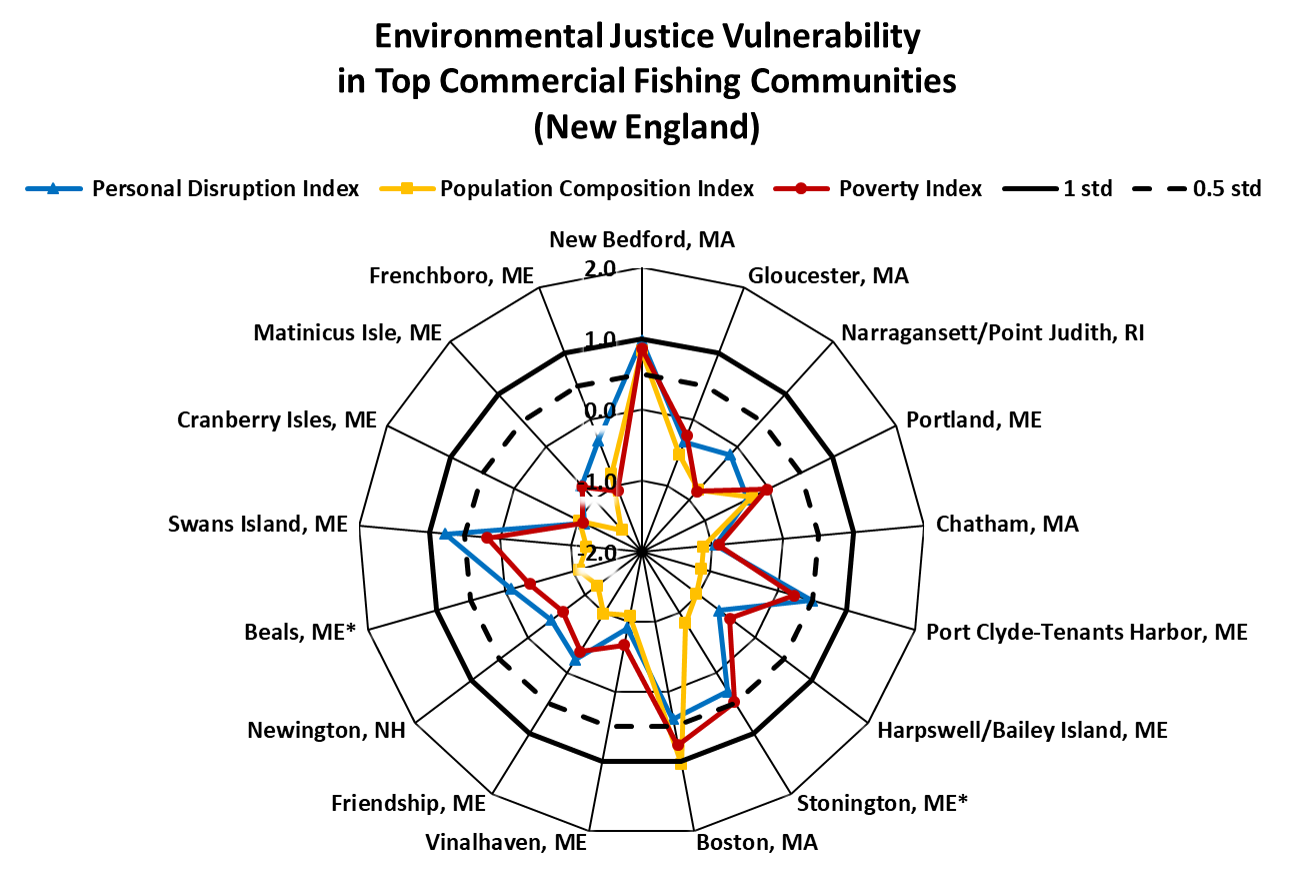
\includegraphics[width=0.75\linewidth]{SOE-NEFMC_files/figure-latex/commercial-EJ-1} 

}

\caption{Environmental justice indicators (Poverty Index, population composition index, and personal disruption index) for top commercial fishing communities in New England. *Community scored high (1.00 and above) for both commercial engagement and reliance indicators.}\label{fig:commercial-EJ}
\end{figure}

No communities in New England scored high for both recreational engagement and reliance (Fig.\ref{fig:recreational-engagement}). All of the top recreational communities scored lower than medium-high for all of the three environmental justice indicators, meaning that environmental justice may not be a major concern in these communities at this time, based on this particular analysis.

Fig. \ref{fig:recreational-EJ} orders communities clockwise in a descending order of recreational engagement scores from high to low, with the most highly engaged community, Narragansett/Point Judith, RI, listed on the top. Narragansett/Point Judith, like all of these top recreational communities ranked low for environmental justice vulnerability. In fact, the scores below 0 for all three environmental justice indicators implies a lower than average level of vulnerability, based on recreational engagement and reliance, among the communities included in the analysis.

\begin{figure}

{\centering \includegraphics{SOE-NEFMC_files/figure-latex/recreational-engagement-1} 

}

\caption{Recreational engagement and reliance, and environmental justice vulnerability, for the top recreationally engaged and reliant fishing communities in New England. None of these communities ranked medium-high or above for one or more of the environmental justice indicators.}\label{fig:recreational-engagement}
\end{figure}

\begin{figure}

{\centering 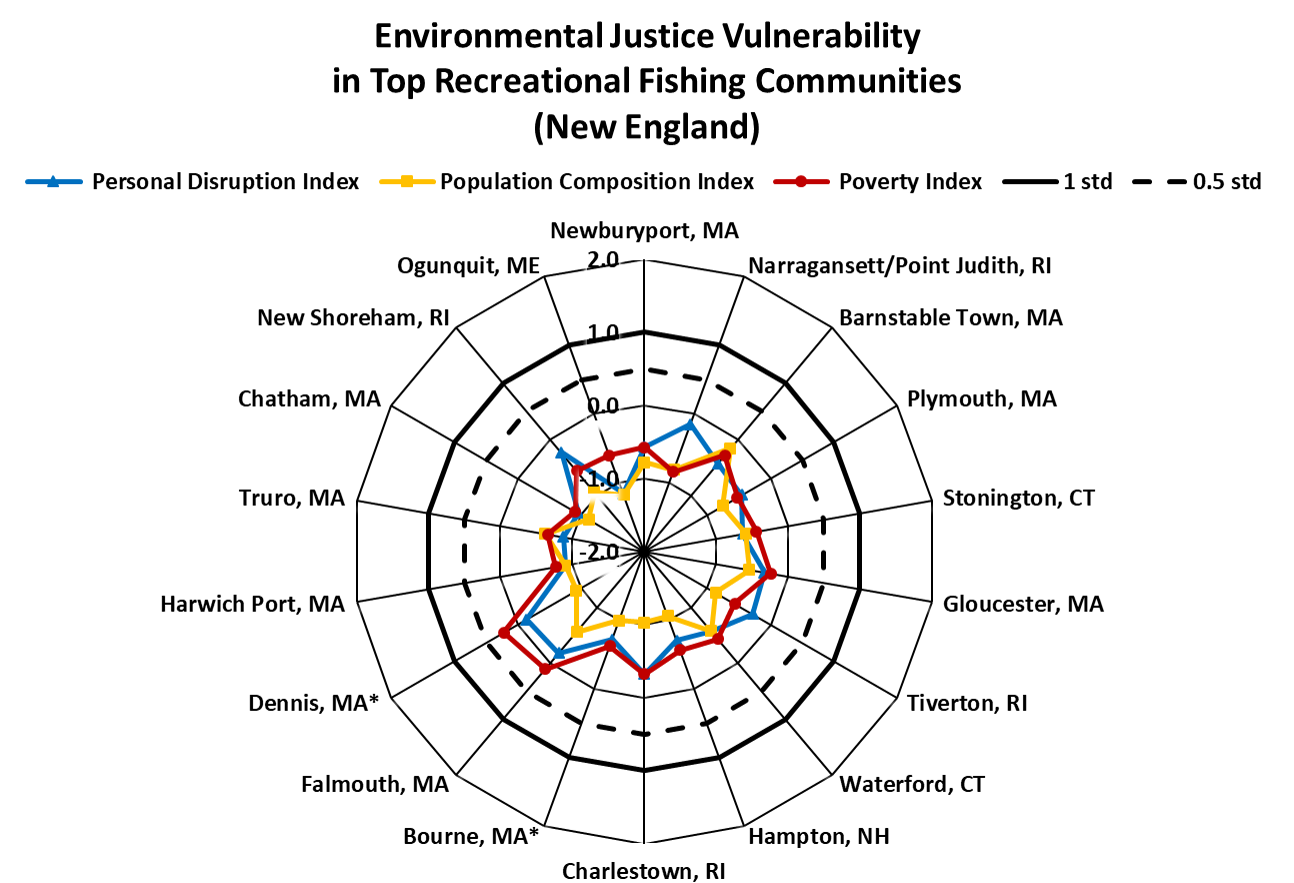
\includegraphics[width=0.75\linewidth]{SOE-NEFMC_files/figure-latex/recreational-EJ-1} 

}

\caption{Environmental justice indicators (Poverty Index, population composition index, and personal disruption index) for top recreational fishing communities in New England. *Community scored high (1.00 and above) for both commercial engagement and reliance indicators.}\label{fig:recreational-EJ}
\end{figure}

Both commercial and recreational fishing are important activities in Narragansett/Point Judith, RI; Gloucester, MA; and Newington, NH, meaning these communities may be impacted simultaneously by commercial and recreational regulatory changes. These three communities currently score low for all of the three environmental justice indicators, indicating that environmental justice may not be a major concern in these communities at the moment based on the indicators analyzed.

\hypertarget{implications-4}{%
\subsubsection{Implications}\label{implications-4}}

These plots provide a snapshot of the presence of environmental justice issues in the most highly engaged and most highly reliant commercial and recreational fishing communities in New England. These communities may be vulnerable to changes in fishing patterns due to regulations and/or climate change. When any of these communities are also experiencing social vulnerability including environmental justice issues, they may have lower ability to successfully respond to change.

\hypertarget{protected-species}{%
\subsection{Protected Species}\label{protected-species}}

Protected species include marine mammals protected under the Marine Mammal Protection Act, endangered and threatened species protected under the Endangered Species Act, and migratory birds protected under the Migratory Bird Treaty Act. In the Northeast U.S., endangered/threatened species include Atlantic salmon, Atlantic and shortnose sturgeon, all sea turtle species, and five baleen whales. Fishery management objectives for protected species generally focus on reducing threats and on habitat conservation/restoration. Here we report on the status of these actions as well as indicating the potential for future interactions driven by observed and predicted ecosystem changes in the Northeast U.S. Protected species objectives include managing bycatch to remain below potential biological removal (PBR) thresholds, recovering endangered populations, and monitoring unusual mortality events (UMEs).

\hypertarget{indicators-bycatch-population-adult-and-juvenile-numbers-mortalities}{%
\subsubsection{Indicators: bycatch, population (adult and juvenile) numbers, mortalities}\label{indicators-bycatch-population-adult-and-juvenile-numbers-mortalities}}

Average indices for both harbor porpoise (Fig. \ref{fig:harborporpoise}) and gray seal bycatch (Fig. \ref{fig:grayseal}) are below current PBR thresholds, meeting management objectives. However, the 2019 bycatch estimate for gray seals was the highest in the time series.

\begin{figure}

{\centering \includegraphics{SOE-NEFMC_files/figure-latex/harborporpoise-1} 

}

\caption{Harbor porpoise average bycatch estimate for Mid-Atlantic and New England gillnet fisheries (blue) and the potential biological removal (red).}\label{fig:harborporpoise}
\end{figure}

\begin{figure}

{\centering \includegraphics{SOE-NEFMC_files/figure-latex/grayseal-1} 

}

\caption{Gray Seal average bycatch estimate for gillnet fisheries (blue) and and the potential biological removal (red).}\label{fig:grayseal}
\end{figure}

The annual estimate for gray seal bycatch has declined since 2019, in part driven by declining gillnet landings. In addition, estimates since 2019 have greater uncertainty stemming from low observer coverage since 2019. The rolling mean confidence interval remains just below the removal threshold.

The North Atlantic right whale population was on a recovery trajectory until 2010, but has since declined (Fig. \ref{fig:narw-abundance}). Reduced survival rates of adult females and diverging abundance trends between sexes have also been observed. It is estimated that there are fewer than 70 adult females remaining in the population.

\begin{figure}

{\centering \includegraphics{SOE-NEFMC_files/figure-latex/narw-abundance-1} 

}

\caption{Estimated North Atlanic right whale abundance on the Northeast Shelf.}\label{fig:narw-abundance}
\end{figure}

North Atlantic right whale calf counts have generally declined after 2009 to the point of having zero new calves observed in 2018 (Fig. \ref{fig:NARW-calf-abundance}). However, since 2019, we have seen more calf births each year with 20 births in 2022.

This year, the Unusual Mortality Event (UME) for North Atlantic right whales continued. Since 2017, the total UME right whale mortalities includes 35 dead stranded whales, 14 in the US and 21 in Canada. When alive but seriously injured whales (22) and sublethal injuries or ill whales (37) are taken into account, 94 individual whales are included in the UME. Recent research suggests that many mortalities go unobserved and the true number of mortalities are about three times the count of the observed mortalities {[}\protect\hyperlink{ref-pace_cryptic_2021}{3}{]}. The primary cause of death is ``human interaction'' from entanglements or vessel strikes\footnote{\url{https://www.fisheries.noaa.gov/national/marine-life-distress/2017-2022-north-atlantic-right-whale-unusual-mortality-event}}.

A UME continued from previous years for humpback whales (2016-present); suspected causes include human interactions. A UME for both gray and harbor seals on the Maine coast was declared in June 2022 due to a high number of mortalities thought to be caused by highly pathogenic avian influenza virus. A UME for minke whales that began in 2017 remains open, but is pending closure as of January 2023\footnote{\url{https://www.fisheries.noaa.gov/national/marine-life-distress/active-and-closed-unusual-mortality-events}}.

\begin{figure}

{\centering \includegraphics{SOE-NEFMC_files/figure-latex/NARW-calf-abundance-1} 

}

\caption{Number of North Atlantic right whale calf births, 1990 - 2021.}\label{fig:NARW-calf-abundance}
\end{figure}

\hypertarget{implications-5}{%
\subsubsection{Implications}\label{implications-5}}

Bycatch management measures have been implemented to maintain bycatch below PBR thresholds. The downward trend in harbor porpoise bycatch can also be due to a decrease in harbor porpoise abundance in US waters, reducing their overlap with fisheries, and a decrease in gillnet effort. The increasing trend in gray seal bycatch may be related to an increase in the gray seal population (U.S. pup counts).

The number of gray seals in U.S. waters has risen dramatically in the last three decades. Based on a survey conducted in 2016, the size of the gray seal population in the U.S. during the breeding season was approximately 27,000 animals, while in Canada the population was estimated to be roughly 425,000. The population in Canada is increasing at roughly 4\% per year, and contributing to rates of increase in the U.S., where the number of pupping sites has increased from one in 1988 to nine in 2019. Mean rates of increase in the number of pups born at various times since 1988 at four of the more data-rich pupping sites (Muskeget, Monomoy, Seal, and Green Islands) ranged from no change on Green Island to high rates of increase on the other three islands, with a maximum increase of 26.3\% (95\%CI: 21.6 - 31.4\%; {[}\protect\hyperlink{ref-wood_rates_2020}{4}{]} Fig. \ref{fig:seals}). These high rates of increase provide further support for the hypothesis that seals from Canada are continually supplementing the breeding population in U.S. waters.

\begin{figure}

{\centering \includegraphics{SOE-NEFMC_files/figure-latex/seals-1} 

}

\caption{Estimated mean rates of increase in the number of gray seal pups born at four United States pupping colonies at various times from 1988 to 2021. Recreated from Wood et al. 2022 (Figure 5).}\label{fig:seals}
\end{figure}

Strong evidence exists to suggest that interactions between right whales and both the fixed gear fisheries in the U.S. and Canada and vessel strikes in the U.S. are contributing substantially to the decline of the species {[}\protect\hyperlink{ref-hayes_north_2018}{5}{]}. Further, right whale distribution has changed since 2010. New research suggests that recent climate driven changes in ocean circulation have resulted in right whale distribution changes driven by increased warm water influx through the Northeast Channel, which has reduced the primary right whale prey (\emph{Calanus finmarchicus}) in the central and eastern portions of the Gulf of Maine {[}\protect\hyperlink{ref-hayes_north_2018}{5}--\protect\hyperlink{ref-sorochan_north_2019}{7}{]}. Additional potential stressors include offshore wind development, which overlaps with important habitat areas used year-round by right whales, including mother and calf migration corridors and foraging habitat. This area is also a primary right whale winter foraging habitat. Additional information can be found in the \protect\hyperlink{other-ocean-uses:-offshore-wind}{offshore wind section}.

The UMEs are under investigation and are likely the result of multiple drivers. For all large whale UMEs, human interaction appears to have contributed to increased mortalities, although investigations are not complete. An investigation into the cause of the seal UME so far suggests avian flu virus as a potential cause.

A climate vulnerability assessment is currently underway for Atlantic and Gulf of Mexico marine mammal populations and will be reported in future versions of this report.

\newpage

\hypertarget{risks-to-meeting-fishery-management-objectives}{%
\section{Risks to meeting fishery management objectives}\label{risks-to-meeting-fishery-management-objectives}}

\hypertarget{climate-and-ecosystem-change}{%
\subsection{Climate and Ecosystem Change}\label{climate-and-ecosystem-change}}

Regulations and measures designed to meet fishery management objectives are often based on historical information about stocks: their distribution in space and time, and their overall productivity. Large scale climate related changes in the ecosystem can lead to changes in important habitats and ecological interactions, altering distributions and productivity. With large enough ecosystem changes, management measures may be less effective, and management objectives may not be met.

This year, we have restructured this section to focus on three categories of management decisions and the risk posed to them by climate and ecosystem change: spatial management, seasonal management, and quota setting or rebuilding depleted stocks. In each section, we highlight observed changes in distribution, timing, and productivity of fish and protected species. Then, we review possible drivers for these observed changes, in order to determine how management might be adjusted to account for the observed changes. Finally, we provide an overview of notable climate and ecosystem observations from 2023.

\hypertarget{risks-to-spatial-management}{%
\subsubsection{Risks to Spatial Management}\label{risks-to-spatial-management}}

Shifting species distributions alter both species interactions and fishery interactions. In particular, shifting species distributions can alter expected management outcomes from spatial allocations and bycatch measures based on historical fish and protected species distributions. Species availability to surveys can change as distributions shift within survey footprints.

\hypertarget{observations-fish-and-protected-species-distribution-shifts}{%
\paragraph{Observations: Fish and protected species distribution shifts}\label{observations-fish-and-protected-species-distribution-shifts}}

As noted in the \protect\hyperlink{implications}{Landings Implications section above}, trends for a suite of 48 commercially or ecologically important fish species along the entire Northeast Shelf continue to show movement towards the northeast and generally into deeper water (Fig. \ref{fig:species-dist}). Habitat model-based species richness suggests shifts of both cooler and warmer water species to the northeast {[}\emph{link to catalog page}{]}. Similar patterns have been found for marine mammals, with multiple species shifting northeast between 2010 and 2017 in most seasons (Fig. \ref{fig:protectedspp-dist-shifts}, {[}\protect\hyperlink{ref-chavez-rosales_detection_2022}{8}{]}).

\begin{figure}

{\centering \includegraphics{SOE-NEFMC_files/figure-latex/protectedspp-dist-shifts-1} 

}

\caption{Direction and magnitude of core habitat shifts, represented by the length of the line of the seasonal weighted centroid for species with more than 70 km difference between 2010 and 2017 (tip of arrow).}\label{fig:protectedspp-dist-shifts}
\end{figure}

\hypertarget{drivers}{%
\paragraph{Drivers:}\label{drivers}}

Increasing temperature, changing oceanography, and the decreasing size of the seasonal cold pool can alter the spatial distribution of suitable habitat for managed species, as well as availability and distribution of their prey.

Ocean temperatures continue to warm at both the surface (Fig. \ref{fig:seasonal-oisst-anom}) and bottom (Fig. \ref{fig:bottom-temp}) throughout Georges Bank and the Gulf of Maine in all seasons.

\begin{figure}

{\centering \includegraphics{SOE-NEFMC_files/figure-latex/seasonal-oisst-anom-1} 

}

\caption{GB and GOM seasonal sea surface temperature (SST) time series . Seasons are defined as: Jan-Mar for winter, Apr-Jun for spring, Jul-Sep for summer, and Oct-Dec for fall.}\label{fig:seasonal-oisst-anom}
\end{figure}

\begin{figure}

{\centering \includegraphics{SOE-NEFMC_files/figure-latex/bottom-temp-1} 

}

\caption{MAB seasonal bottom temperature (BT) anomaly time series. Seasons are defined as: Jan-Mar for winter, Apr-Jun for spring, Jul-Sep for summer, and Oct-Dec for fall.}\label{fig:bottom-temp}
\end{figure}

Variability of the Gulf Stream is one of the major drivers of changes in the oceanographic conditions of the Northeast U.S. continental shelf. During the last decade, the Gulf Stream has become less stable and shifted northward (Fig. \ref{fig:GSI}). A more northern Gulf Stream position is associated with warmer ocean temperature on the northeast shelf {[}\protect\hyperlink{ref-zhang_role_2007}{9}{]}, a higher proportion of Warm Slope Water in the Northeast Channel, and increased sea surface height along the U.S. east coast {[}\protect\hyperlink{ref-goddard_extreme_2015}{10}{]}.

\begin{figure}

{\centering \includegraphics{SOE-NEFMC_files/figure-latex/GSI-1} 

}

\caption{Index representing changes in the location of the Gulf Stream north wall. Positive values represent a more northerly Gulf Stream position.}\label{fig:GSI}
\end{figure}

Since 2008, the Gulf Stream has moved closer to the Grand Banks, reducing the supply of cold, fresh, and oxygen-rich Labrador Current waters to the Northwest Atlantic Shelf {[}\protect\hyperlink{ref-goncalves_neto_changes_2021}{11}{]}. Nearly every year since 2010, warm slope water made up more than 75\% of the annual slope water proportions entering the Gulf of Maine. In 2017 and 2019, almost no cooler Labrador Slope water entered the Gulf of Maine through the Northeast Channel (Fig. \ref{fig:wsw-prop}). The changing proportions of source water affect the temperature, salinity, and nutrient inputs to the Gulf of Maine ecosystem. In 2021, warm slope water continued to dominate (86.1\%) inputs to the Gulf of Maine.

\begin{figure}

{\centering \includegraphics{SOE-NEFMC_files/figure-latex/wsw-prop-1} 

}

\caption{Proportion of Warm Slope Water (WSW) and Labrador slope water (LSLW) entering the GOM through the Northeast Channel.}\label{fig:wsw-prop}
\end{figure}

Changes in the distribution of forage biomass affects predator distribution. Spatial subsets of the forage fish index were included in the bluefish research track stock assessment to investigate forage-driven changes in bluefish availability to recreational fisheries and surveys.

\hypertarget{risks-to-seasonal-management}{%
\subsubsection{Risks to Seasonal Management}\label{risks-to-seasonal-management}}

Changes in seasonal life-cycle events may not align with fishing seasons or area opening/closing, potentially reducing effectiveness of management measures. Temporal changes in species/fishery overlap can alter bycatch, and availability to surveys can change.

\hypertarget{observations-timing-shifts}{%
\paragraph{Observations: Timing shifts}\label{observations-timing-shifts}}

Seasonal timing of spawning has changed for several managed fish species. Migration timing of some tunas and large whales has changed.

GENERATE A FIGURE

\hypertarget{drivers-1}{%
\paragraph{Drivers:}\label{drivers-1}}

Later transition to fall conditions, shorter duration of seasonal cold pool, changing timing of fall phytoplankton blooms, seasonal community shifts in zooplankton, and changes in timing of food availability contribute to changes in species timing.

In addition to increasing seasonal temperatures, ocean summer conditions now last longer within each year. In both GB and GOM, the transition date from cool winter conditions to warm stratified summer conditions is getting earlier. The transition back to well mixed cool temperatures is also getting later in the year, thus increasing the total number of days when the surface temperatures are in the warm summer conditions (Fig. \ref{fig:transition}).

\begin{figure}

{\centering \includegraphics{SOE-NEFMC_files/figure-latex/transition-1} 

}

\caption{Ocean summer length in the MAB: the annual total number of days between the spring thermal transition date and the fall thermal transition date.  The transition dates are defined as the day of the year when surface temperatures changeover from cool to warm conditions in the spring and back to cool conditions in the fall.}\label{fig:transition}
\end{figure}

Cold pool timing has changed in the Mid-Atlantic, with the feature persisting for a shorter portion of the year since the mid-2000s (Fig. \ref{fig:cold-pool-time}). \emph{IMPACTS TO NEW ENGLAND SPAWNERS?}

\begin{figure}

{\centering \includegraphics{SOE-NEFMC_files/figure-latex/cold-pool-time-1} 

}

\caption{Seasonal cold pool indices: mean temperature within the cold pool, cold pool persistence, and spatial extent.}\label{fig:cold-pool-time}
\end{figure}

\hypertarget{risks-to-quota-settingrebuilding}{%
\subsubsection{Risks to Quota Setting/Rebuilding}\label{risks-to-quota-settingrebuilding}}

Environmentally driven changes in growth, reproduction, and natural mortality can complicate short-term stock projections. Stock reference points may not reflect prevailing environmental conditions.

\hypertarget{observations-fish-productivity-and-condition-shifts}{%
\paragraph{Observations: Fish productivity and condition shifts}\label{observations-fish-productivity-and-condition-shifts}}

We describe patterns of aggregate fish productivity in the Mid-Atlantic with the small fish per large fish anomaly indicator, derived from NEFSC bottom trawl survey data (Fig. \ref{fig:productivity-anomaly}). The indicator shows that productivity has been declining in this region since the early 2000s. A similar analysis based on stock assessment model outputs (recruitment per spawning stock biomass anomaly) for stocks primarily inhabiting the Mid-Atlantic region also shows a decline in productivity.

\begin{figure}

{\centering \includegraphics{SOE-NEFMC_files/figure-latex/productivity-anomaly-1} 

}

\caption{Fish productivity measures. Left: Small fish per large fish survey biomass anomaly in the Mid-Atlantic Bight. Right: assessment recruitment per spawning stock biomass anomaly for stocks mainly in the Mid-Atlantic. The summed anomaly across species is shown by the black line, drawn across all years with the same number of stocks analyzed.}\label{fig:productivity-anomaly}
\end{figure}

The health and well being of individual fish can determine population productivity. Heavier and fatter fish at a given length have higher relative condition (the ratio of observed weight to predicted weight based on length {[}\protect\hyperlink{ref-le_cren_length-weight_1951}{12}{]}) which is expected to improve growth, reproductive output, and survival. A pattern of generally good condition was observed across many species prior to 2000, followed by a period of generally poor condition from 2001-2010 (concurrent with declines in productivity, Fig. \ref{fig:productivity-anomaly}), , with a mix of good and poor condition 2011-2019, and improved condition for many species in 2021 and 2022 (Fig. \ref{fig:ne-cf}). Preliminary results of synthetic analyses show that changes in temperature, zooplankton, fishing pressure, and population size influence the condition of different fish species.

\begin{figure}

{\centering \includegraphics{SOE-NEFMC_files/figure-latex/ne-cf-1} 

}

\caption{Condition factor for fish species in New England based on fall NEFSC bottom trawl survey data. No survey was conducted in 2020.}\label{fig:ne-cf}
\end{figure}

\hypertarget{drivers-2}{%
\paragraph{Drivers:}\label{drivers-2}}

Fish productivity and condition are affected by increasing metabolic demands from increasing temperature, combined with changes in the availability and quality of prey. Episodic extreme temperatures, ocean acidification, and low oxygen events represent multiple stressors that can affect growth rates and cause mortality.

\emph{Need to place this} Common tern productivity has also declined in the Gulf of Maine. 2021 and 2023 were challenging years for terns raising chicks (Fig. \ref{fig:seabird-ne-productivity}).

\begin{figure}

{\centering \includegraphics{SOE-NEFMC_files/figure-latex/seabird-ne-productivity-1} 

}

\caption{Productivity of Common terns in the Gulf of Maine.}\label{fig:seabird-ne-productivity}
\end{figure}

want the salmon here? another system productivity symptom?

\begin{center}\includegraphics{SOE-NEFMC_files/figure-latex/unnamed-chunk-2-1} \end{center}

\hypertarget{forage-quality-and-abundance}{%
\subparagraph{Forage quality and abundance}\label{forage-quality-and-abundance}}

The amount of forage fish available in the ecosystem combined with the energy content of the forage species determines the amount of energy potentially available to predators in the ecosystem. Changes in the forage base can drive to managed and protected species production.

Nutritional value (energy content) of juvenile and adult forage fish as prey is related to environmental conditions, fish growth, and reproductive cycles. Forage energy density measurements from NEFSC trawl surveys 2017-2022 are building toward a time series to evaluate trends (Fig. \ref{fig:energy-density}). Data from the fall 2021 and spring 2022 survey measurements were consistent with previous reports: the energy density of Atlantic herring increased to over 7 kJ/g wet weight, but was still well below that observed in the 1980s and 1990s (10.6-9.4 kJ/ g wet weight). Silver hake, longfin squid (\emph{Loligo} in figure) and shortfin squid (\emph{Illex} in figure) remain lower than previous estimates {[}\protect\hyperlink{ref-steimle_energy_1985}{13},\protect\hyperlink{ref-lawson_important_1998}{14}{]}. Energy density of alewife, butterfish, sand lance, and Atlantic mackerel varies seasonally, with seasonal estimates both higher and lower than estimates from previous decades.\\

\begin{figure}

{\centering \includegraphics{SOE-NEFMC_files/figure-latex/energy-density-1} 

}

\caption{Forage fish energy density mean and standard deviation by season and year, compared with 1980s (solid line; Steimle and Terranove 1985) and 1990s (dashed line; Lawson et al. 1998) values.}\label{fig:energy-density}
\end{figure}

A spatially-explicit forage index estimated the combined biomass of 20 forage species using stomach contents information from 22 predatory fish species collected on bottom trawl surveys. The resulting indices show an increasing long term trend in fall the Gulf of Maine, and overall higher forage fish in fall relative to spring (Fig. \ref{fig:foragebio}), with highest forage biomass during fall in the mid-1980s.\\

\begin{figure}

{\centering \includegraphics{SOE-NEFMC_files/figure-latex/foragebio-1} 

}

\caption{Forage fish index based on spring and fall survey predator diets.}\label{fig:foragebio}
\end{figure}

\emph{This is where we would put in overall zooplankton production as well as comments on zoop energy content. Talk about Cal fin availability in New England}
Decadal periodicity in the abundance of dominant copepods in the GOM and on GB has been previously reported, and these patterns continued to evolve into 2021. The abundance of \emph{C. typicus} has been above average since 2012 in the GOM and on GB, and appears to be negatively correlated with \emph{C. finmarchicus} abundance on GB (Fig. \ref{fig:zoo-abund}). \emph{C. finmarchicus} has been below average in abundance since 2012 on GB following a period of high abundance between 2000-2010. \emph{C. finmarchicus} also had high abundance in the GOM between 2000-2010, which corresponded to a period of recovery for right whales (Fig. \ref{fig:narw-abundance}). The abundance of \emph{Pseudocalanus spp.}, an important prey item for cod larvae and other ichthyoplankton, has been below average on GB since 2000 and was below average in the GOM from 2000-2015, and most recently in 2021 the GOM larval fish diversity declined due to high abundance of hake (red, white, and silver) larvae.

\begin{figure}

{\centering \includegraphics{SOE-NEFMC_files/figure-latex/zoo-abund-1} 

}

\caption{Abundance Annomalies of three dominante zooplankton (\textit{Calanus finmarchicus}, \textit{Calanus typicus}, and \textit{Pseudocalanus spp}.) on Georges Bank (GB) and the Gulf of Maine (GOM).}\label{fig:zoo-abund}
\end{figure}

Phytoplankton support the food web as the primary food source for zooplankton and filter feeders such as shellfish. Numerous environmental and oceanographic factors interact to drive the abundance, composition, spatial distribution, and productivity of phytoplankton.

While changes in fish productivity could result from changing primary productivity, total primary production in New England has no clear trend.

\begin{center}\includegraphics{SOE-NEFMC_files/figure-latex/pptot-1} \end{center}

Temperature increases at both the surface (Fig. \ref{fig:seasonal-oisst_anom}) and bottom (Fig. \ref{fig:bottom-temp}) can exceed thermal tolerance limits for some fish. For example, 2012 had among the warmest surface and bottom temperatures in New England. A large proportion of the region had bottom temperatures above the thermal tolerance for groundfish\ldots{} with some days exceeding the mortality limit (Fig. \ref{fig:therm-hab-persist-2012}).

\begin{center}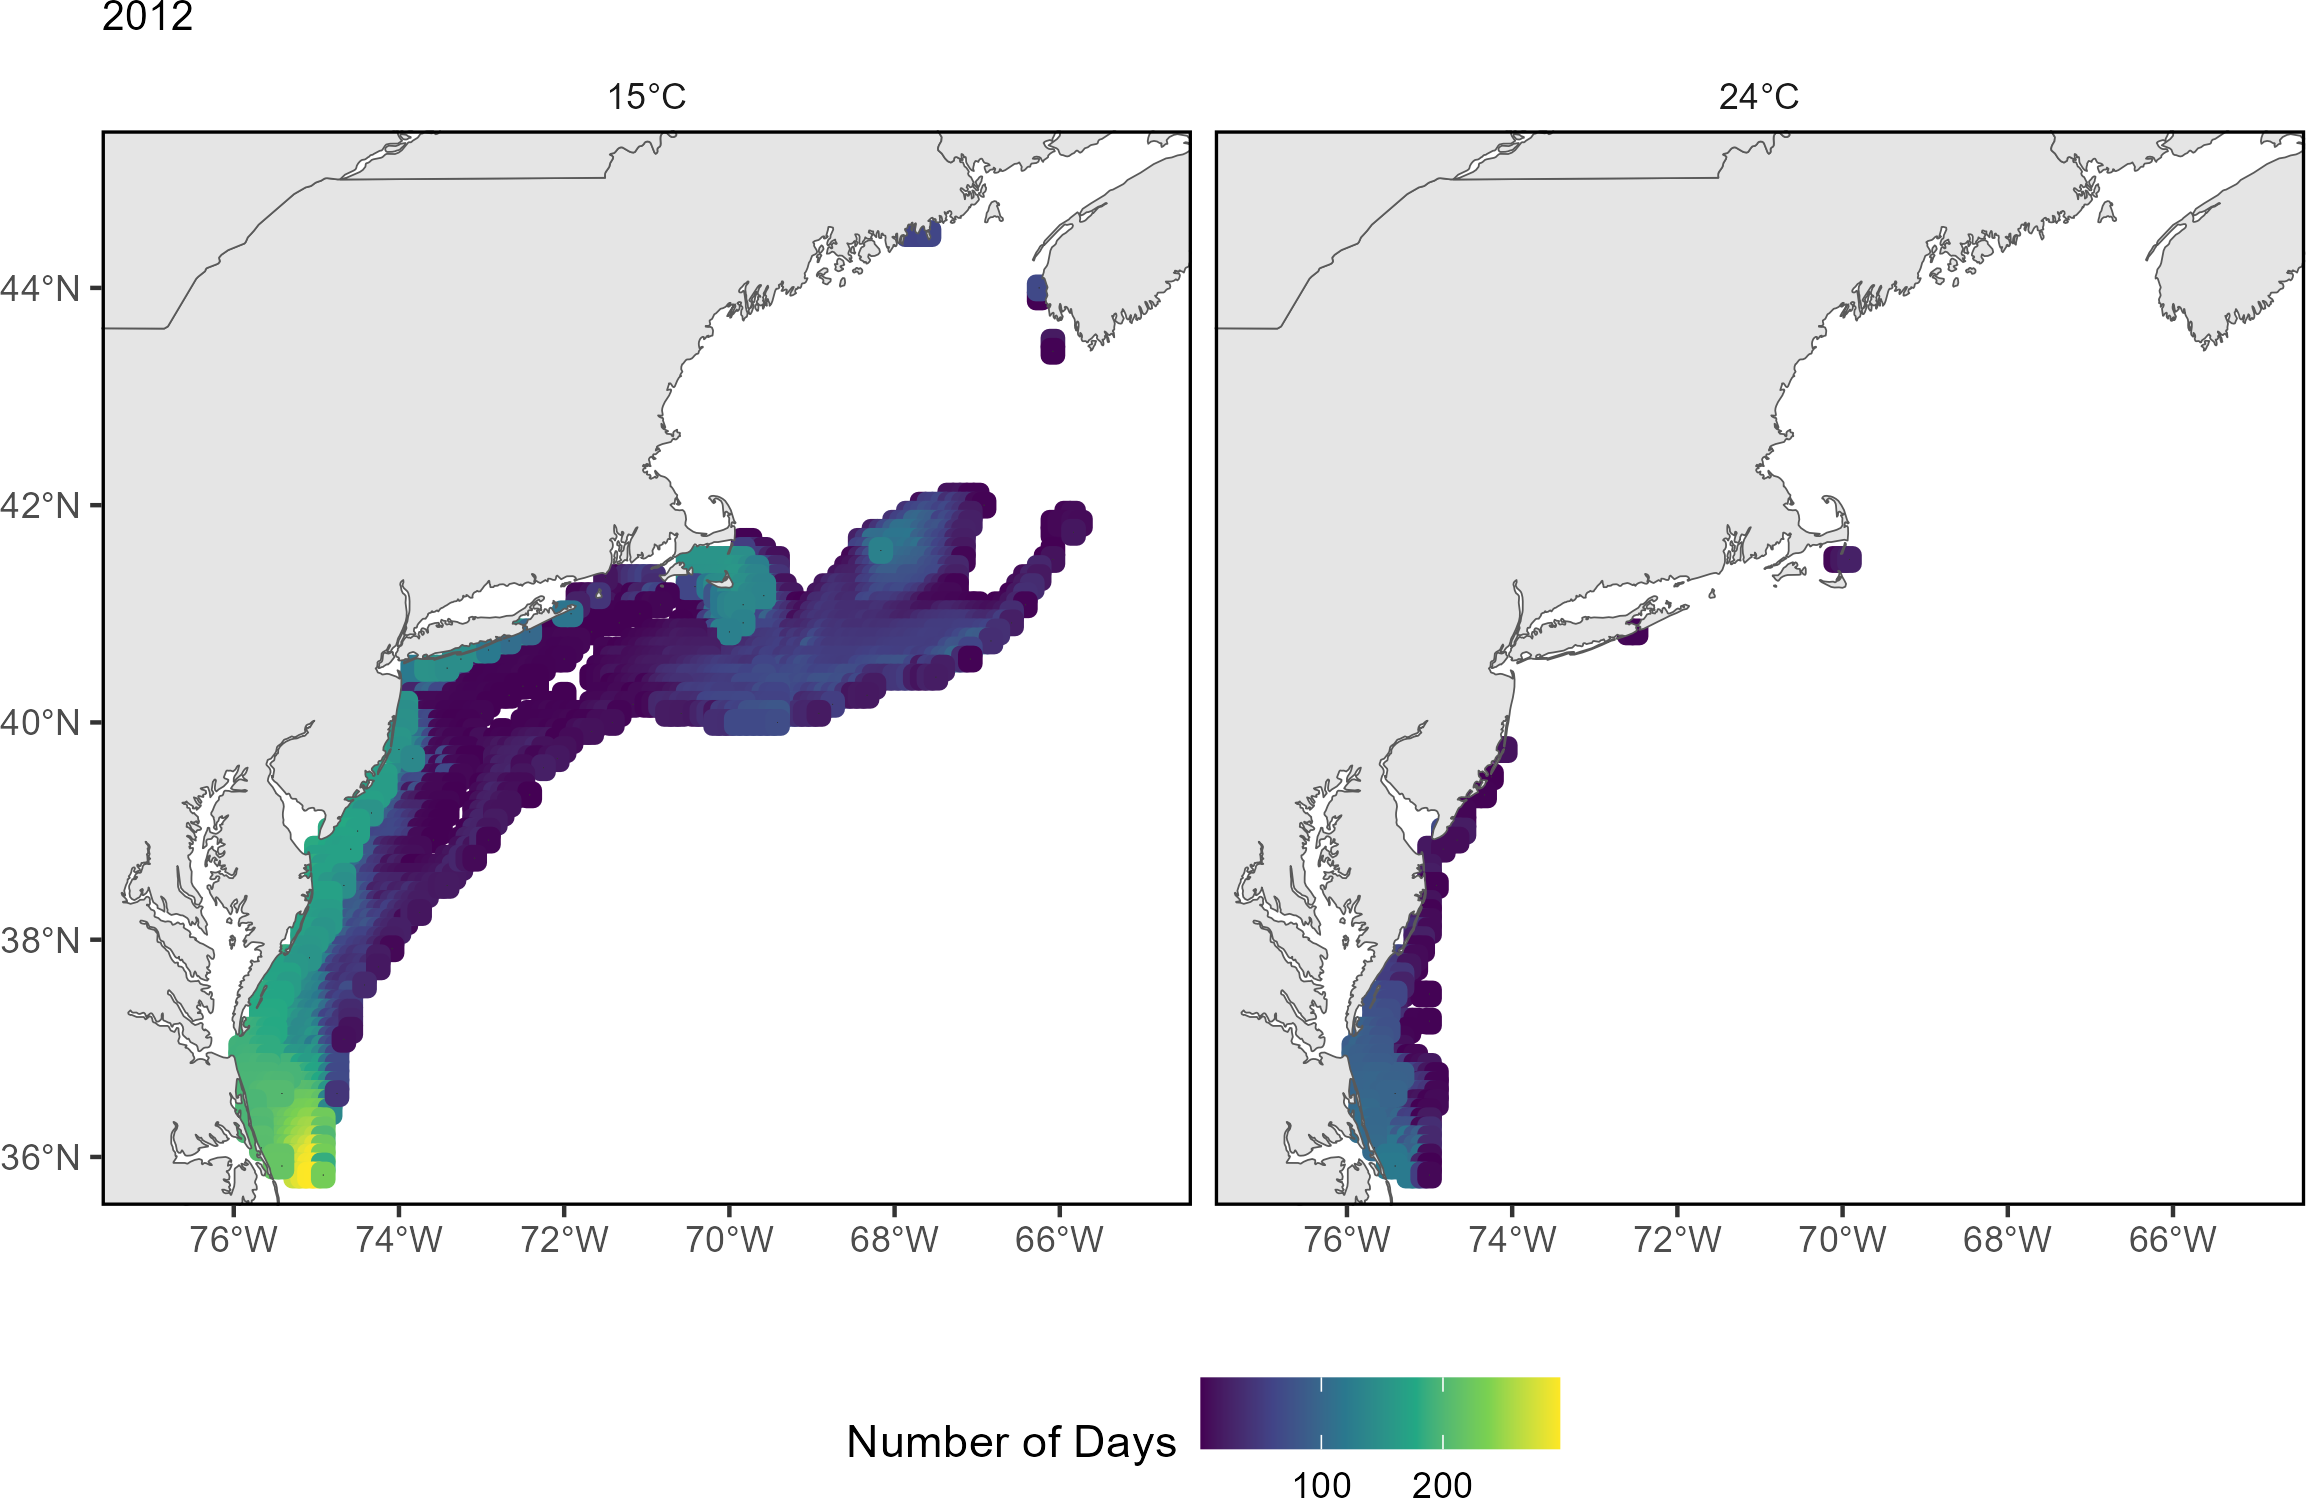
\includegraphics{SOE-NEFMC_files/figure-latex/therm-hab-persist-2012-1} \end{center}

Ocean acidification (OA) has caused measured declines in global ocean pH, and is projected to continue declining if high carbon dioxide emissions continue {[}\protect\hyperlink{ref-intergovernmental_panel_on_climate_change_ipcc_technical_2022}{15}{]}. OA also changes the availability of minerals required by organisms to form calcified structures such as shells. Calcifying conditions in seawater can be determined by measuring aragonite saturation state (\(\Omega_{Arag}\)), the tendency of a common type of calcium carbonate, aragonite, to form or dissolve. When \(\Omega_{Arag}\) is less than 1, shells and other calcium carbonate structures begin to dissolve. Typical surface ocean \(\Omega_{Arag}\) is 2-4, but extremes can be \textless1 or \textgreater5 {[}\protect\hyperlink{ref-jiang_climatological_2015}{16}{]}. As the ocean absorbs carbon dioxide, both pH and \(\Omega_{Arag}\) decrease and can cause organisms to respond with reduced survival, calcification rates, growth, and reproduction, as well as impaired development, and/or changes in energy allocation {[}\protect\hyperlink{ref-saba_recommended_2019}{18}{]}. However, sensitivity levels vary, and some organisms exhibit negative responses to calcification and other processes when \(\Omega_{Arag}\) is as low as 3.

\emph{OLD TEXT REWRITE FOR NEW FIGURES}
Summer-time (2007-present) \(\Omega_{Arag}\) on the U.S. Northeast Shelf varies in space and time, ranging from 0.64 to 2.49 (Fig. \ref{fig:mab-oa}, left panel). Spatially, the lowest bottom \(\Omega_{Arag}\) has occurred in the Gulf of Maine, western Long Island Sound, nearshore to mid-shelf waters of the Mid-Atlantic Bight off the coast of New Jersey, and in waters \textgreater{} 1000 meters. \(\Omega_{Arag}\) was at or below the sensitivity levels for both Atlantic sea scallop {[}\protect\hyperlink{ref-cameron_effects_2022}{19}{]} and longfin squid {[}\protect\hyperlink{ref-zakroff_dose-dependence_2019}{20},\protect\hyperlink{ref-zakroff_antagonistic_2020}{21}{]} in Long Island Sound and the nearshore and mid-shelf regions of the New Jersey shelf (Fig. \ref{fig:mab-oa}, right panels). The sensitivity levels of bottom \(\Omega_{Arag}\) occurred during August 2016, July 2018, and August 2019 for both species, and additionally in August 2021 for the Atlantic sea scallop.

\begin{figure}

{\centering 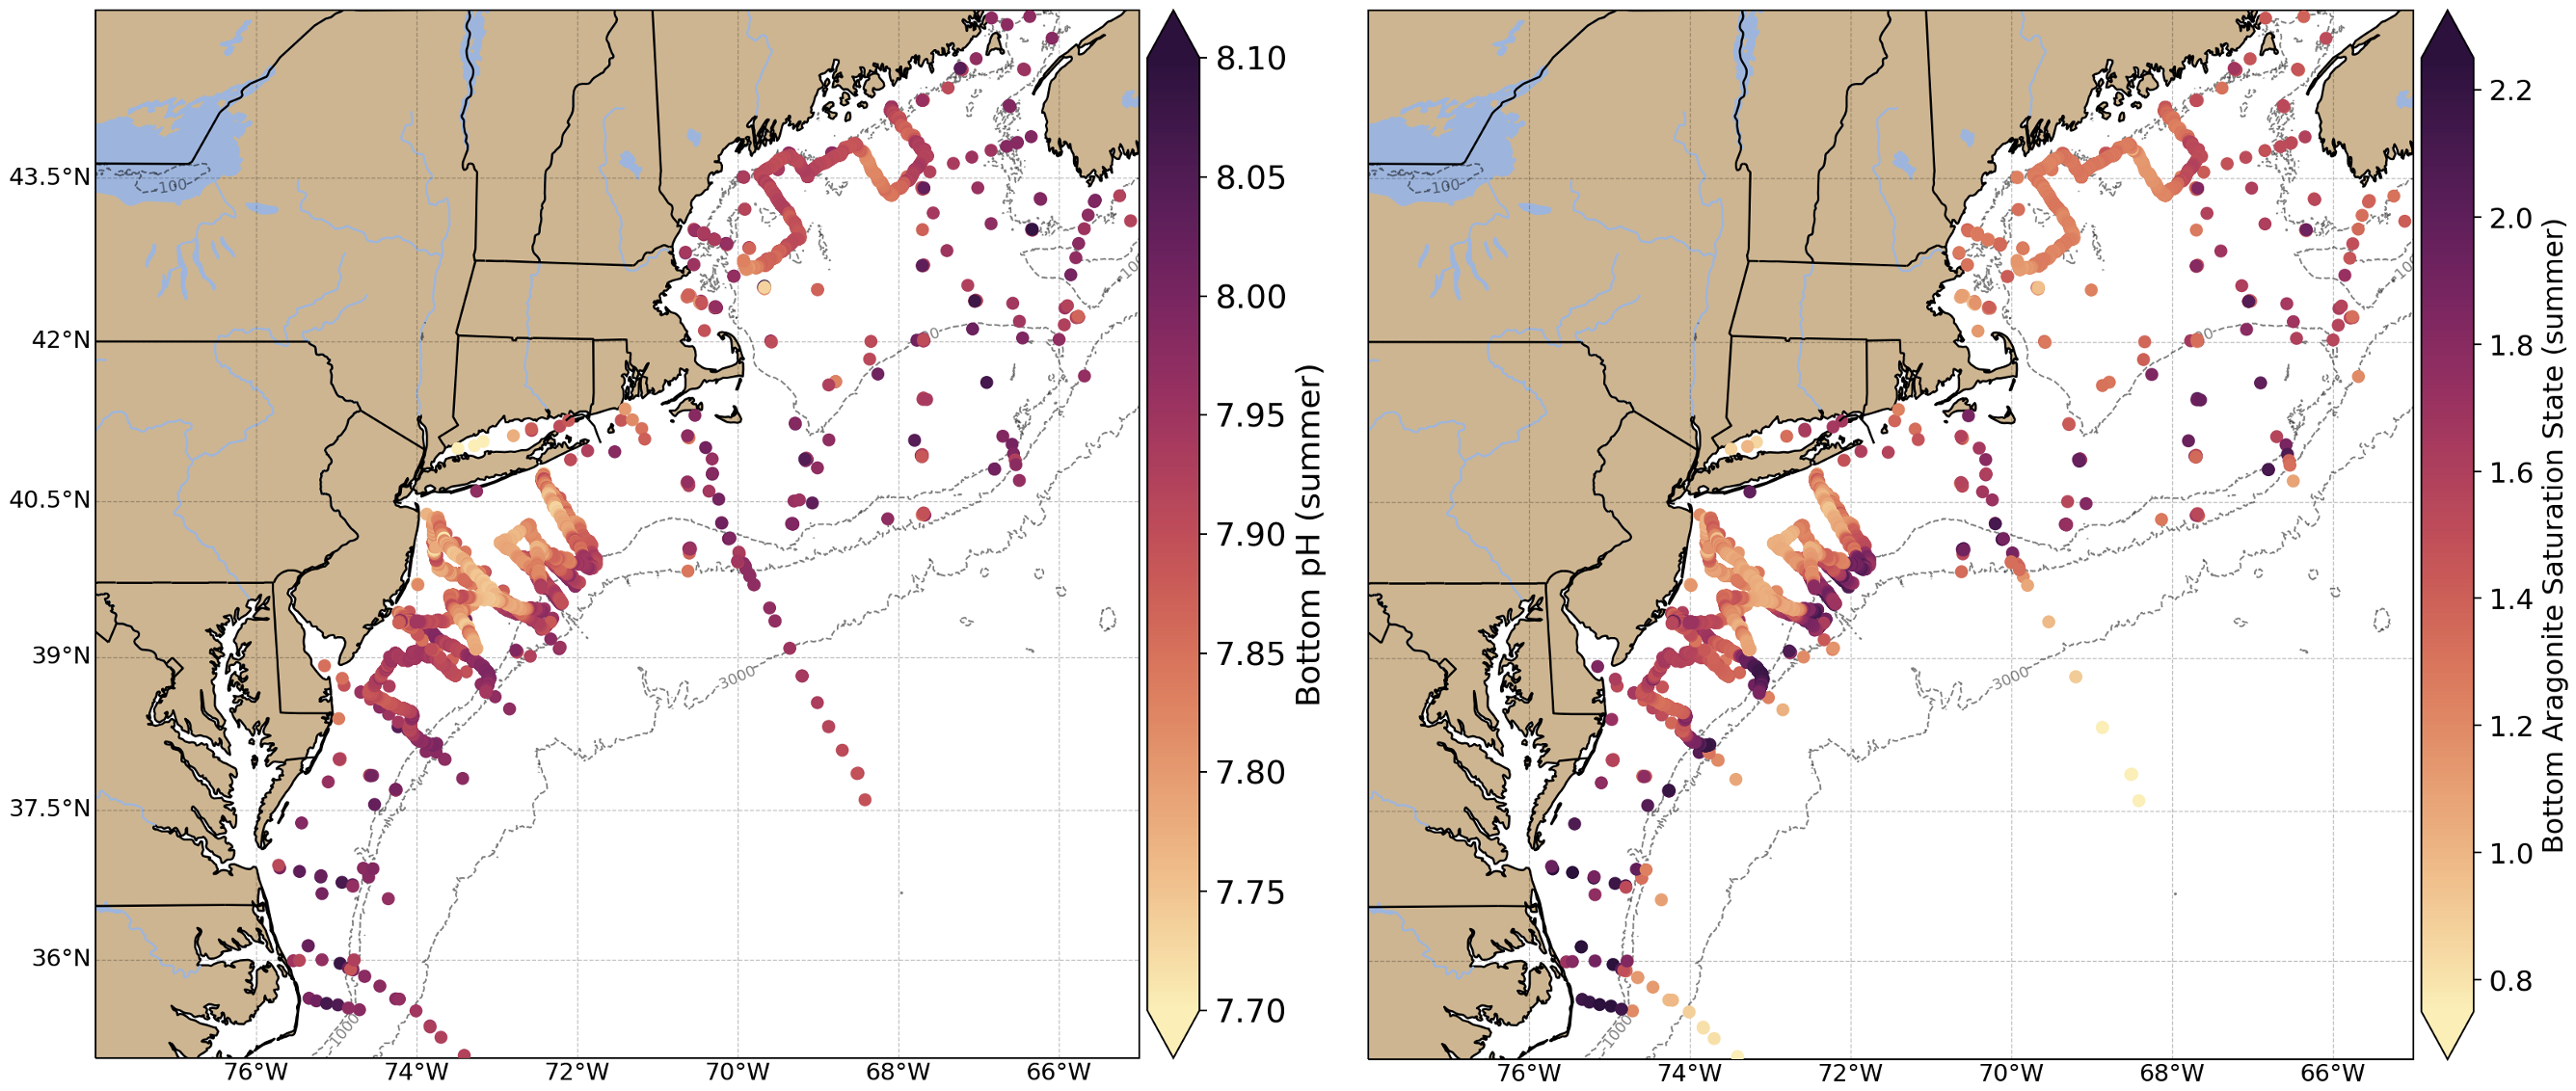
\includegraphics[width=1\linewidth]{SOE-NEFMC_files/figure-latex/mab-oa-1} 

}

\caption{Bottom summer-time (June-August) pH (left panel) and aragonite saturation state (right panel) on the U.S. Northeast Shelf from 2007-2023 plotted from available quality-controlled vessel- and glider-based datasets.}\label{fig:mab-oa}
\end{figure}

\begin{figure}

{\centering 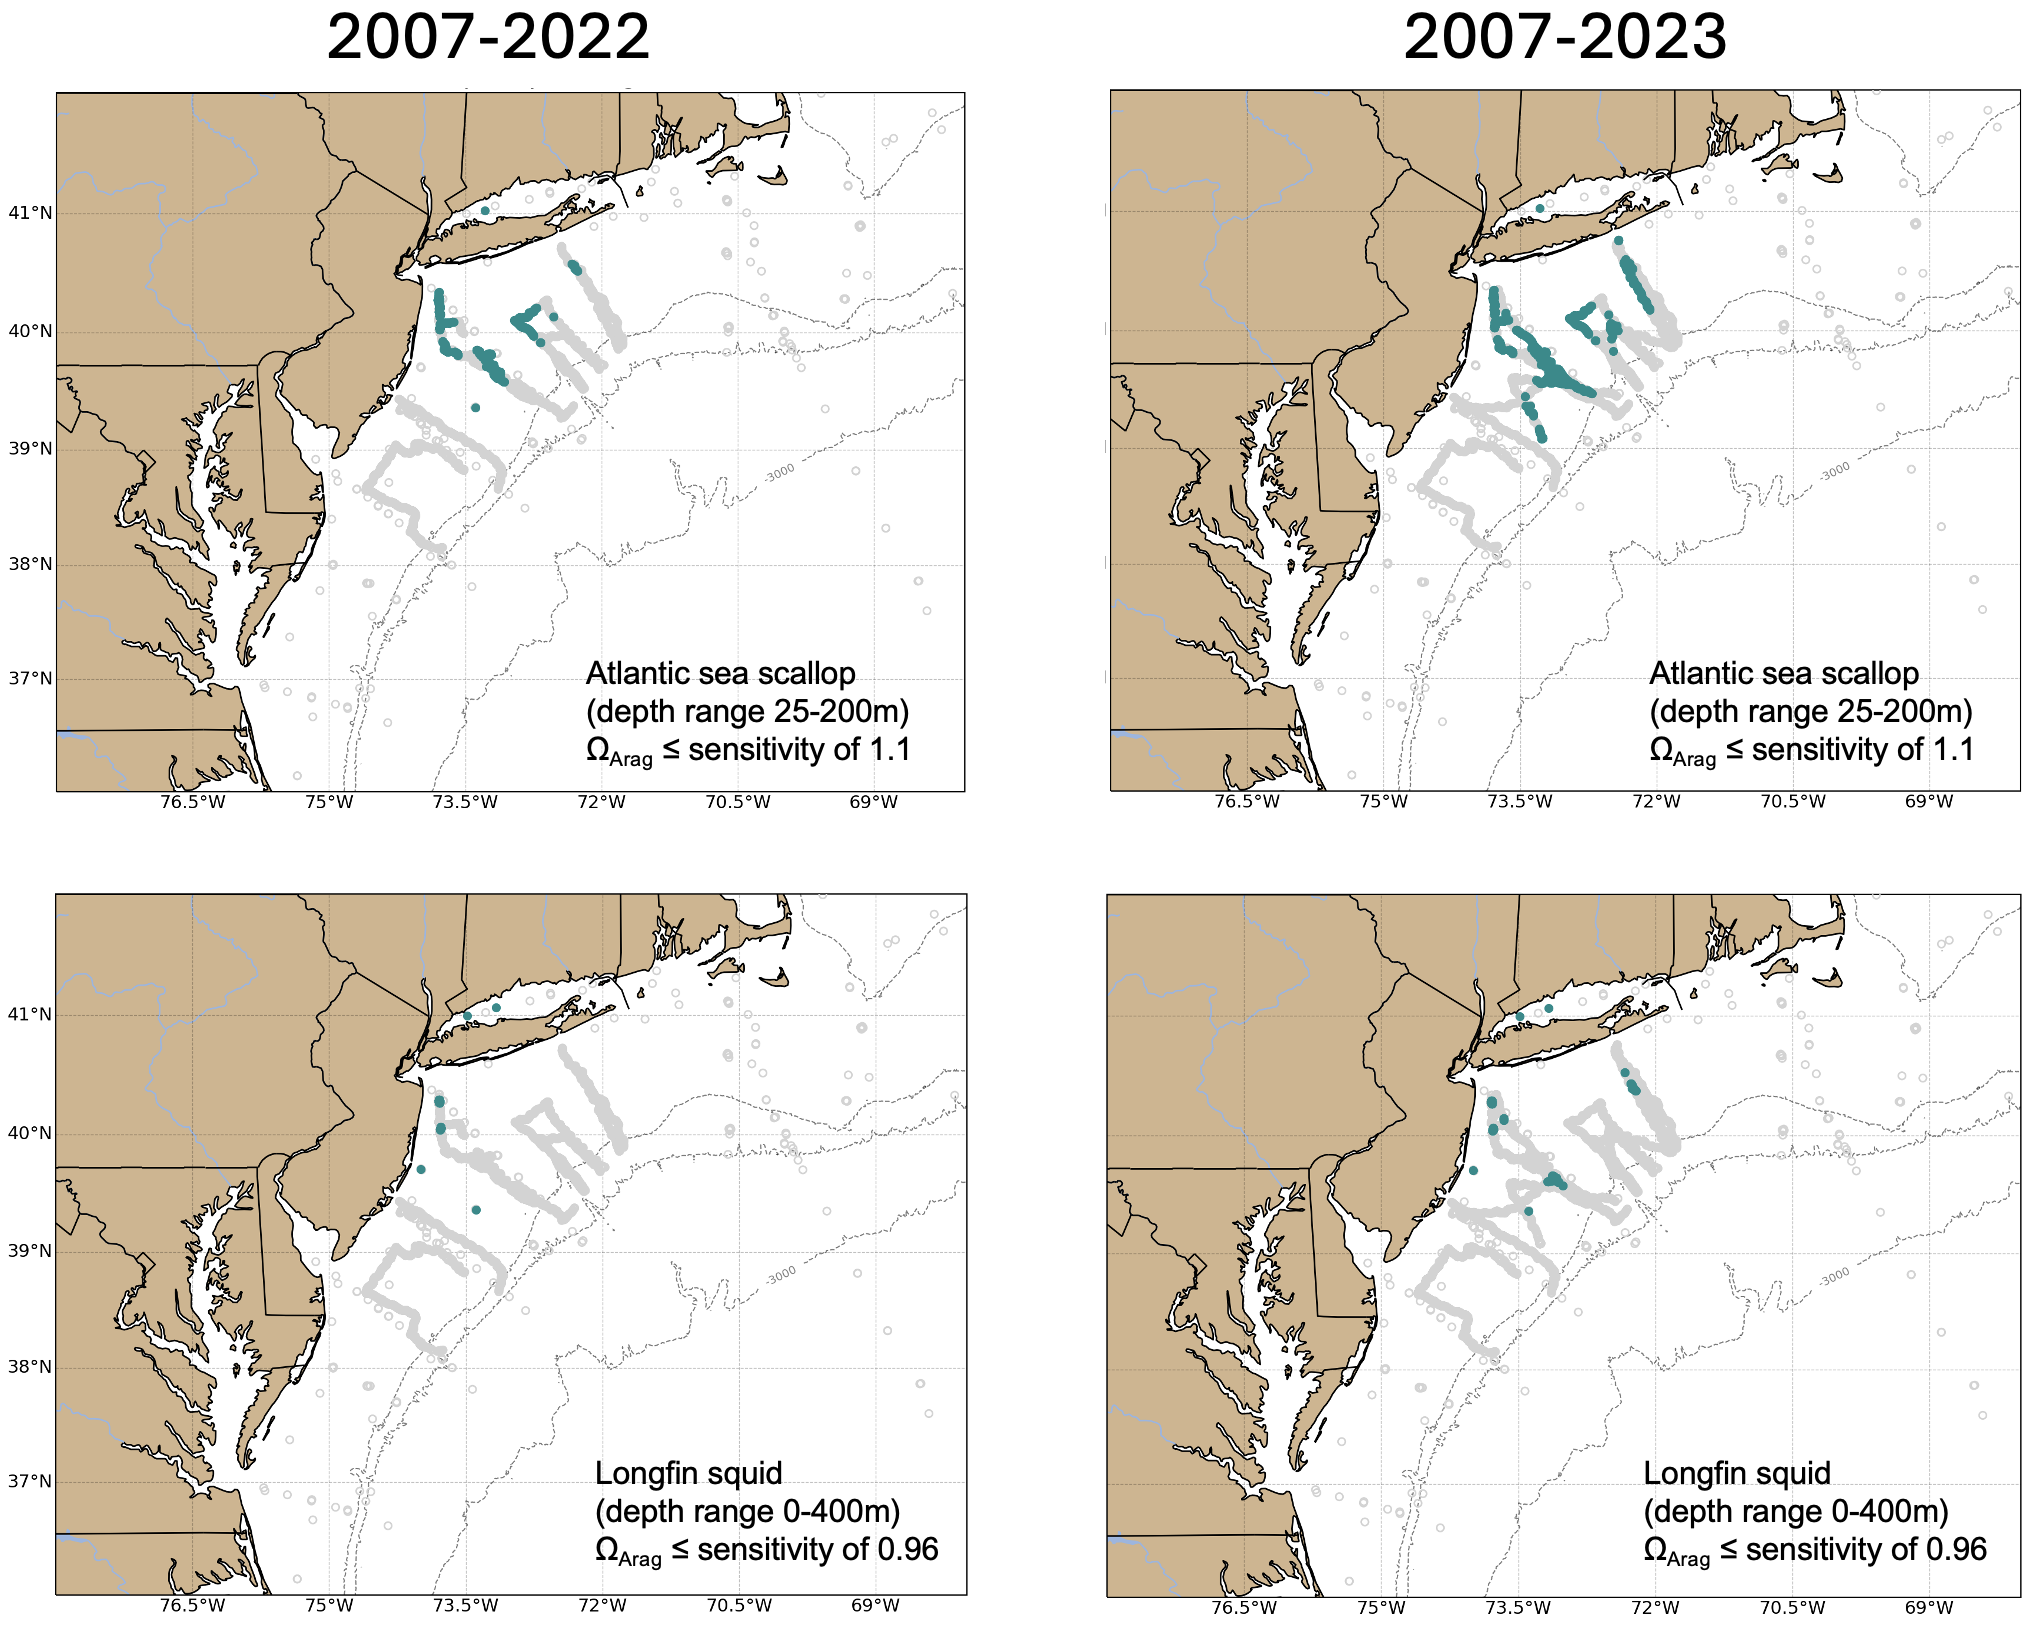
\includegraphics[width=1\linewidth]{SOE-NEFMC_files/figure-latex/oa-spp-1} 

}

\caption{Locations where bottom aragonite saturation state ($\Omega_{Arag}$; summer only: June-August) were at or below the laboratory-derived sensitivity level for Atlantic sea scallop (top panels) and longfin squid (bottom panels) for the time periods 2007-2022 (left panels) and 2007-2023 (right panels). Gray circles indicate locations where carbonate chemistry samples were collected, but bottom $\Omega_{Arag}$ values were higher than sensitivity values determined for that species.}\label{fig:oa-spp}
\end{figure}

Low oxygen events

\hypertarget{current-status-2023-overview}{%
\subsubsection{Current status: 2023 overview}\label{current-status-2023-overview}}

Multiple anomalous conditions and extreme events were observed in 2023 that could have brief local effects and/or widespread long-term ecosystem, fishery and management implications. Reported observations should be noted and taken into consideration for future analyses and assessments.

Globally, 2023 was the warmest year on record with record high global sea surface temperatures. North Atlantic surface temperatures were also the highest on record, however temperatures in the Northeast U.S. shelf ecosystem were more variable, near record highs in winter and near average in other seasons. Chesapeake Bay rarely exceeded temperature thresholds.

Bottom temperatures likely thresholds of X and Y degrees for N days in 2023, especially along the Mid-Atlantic coast. \emph{which species care?}

\begin{center}\includegraphics{SOE-NEFMC_files/figure-latex/therm-hab-persist-2023-1} \end{center}

The 2020-2022 La Niña conditions ended in late winter and shifted to strong El Niño conditions in late spring 2023. The current El Niño is expected to gradually weaken and transition to neutral conditions in spring 2024. During El Niño winters, there is a noted increased frequency of East Coast storms. \emph{add potential implications for fisheries}

Fall tropical and coastal storms caused several flash flood events, above average coastal water levels, strong winds and high rainfall totals throughout the Northeast. \emph{add potential implications for fisheries}

Gulf Stream instability resulted in variability throughout the year. In the fall, the Gulf Stream was in a northward position along the Mid-Atlantic shelf break for an extended period of time. This severely constricted the Slope Sea waters that are normally between the Gulf Stream and continental shelf break. Warm salty surface Gulf Stream waters with strong currents were observed on the continental shelf in the southern MAB in October. \emph{add potential implications for fisheries}

The number of warm core rings (18) was well below the current regime (2000-2022) average of 31. One large early season ring was observed along the Northeast Shelf Break in spring, which generated an anomalously large shelf streamer that pulled continental shelf water into the Slope Sea. \emph{add potential implications for fisheries}

High abundances of large baleen whale species (North Atlantic rRight wWhales and , humpback whales, minke, (others)) were observed feeding near a warm core rings that wereas adjacent to the continental shelf break in spring.
Summer bottom temperatures in the Gulf of Maine were the warmest on record (since 1993) and the second largest bottom marine heatwave occurred from FebruaryMarch to August, peaked in May, and likely continued into the fall (pending data update).

Record high (since 1998) chlorophyll concentrations were up to ten times greater than average during a wide-spread, long-duration phytoplankton bloom in the Gulf of Maine that extended onto Georges Bank and the northern Mid-Atlantic Bight (Fig. \ref{fig:chl-current-year}).

\emph{add potential implications for fisheries: such as:}

A large phytoplankton bloom could represent either an influx of energy into the system, boosting productivity of zooplankton or higher trophic levels, or a settling of unconsumed dead phytoplankton cells to the bottom, where low oxygen could result due to increased bacterial activity consuming the settled material, or both.

NEITHER HAPPENED

It wasn't the typical bloom species.

This species wasn't consumed so we don't expect it to boost fish productivity

This species didn't sink to the bottom so we didn't get low oxygen

\begin{figure}

{\centering \includegraphics{SOE-NEFMC_files/figure-latex/chl-current-year-1} 

}

\end{figure}

Documented die off of scallops in the Mid-Atlantic Elephant trunk regions between the 2022 and 2023 surveys.
A fish and shellfish mortality event was observed in coastal New Jersey linked to hypoxia (low dissolved oxygen) and ocean acidification.

In Chesapeake Bay, hypoxia conditions were the lowest on record (since 1995), creating more suitable habitat for adult and juvenile striped bass.

\hypertarget{implications-6}{%
\subsubsection{Implications}\label{implications-6}}

\emph{SUMMARIZE IMPLICATIONS OF THE WHOLE SECTION}

\hypertarget{other-ocean-uses-offshore-wind}{%
\subsection{Other Ocean Uses: Offshore Wind}\label{other-ocean-uses-offshore-wind}}

\hypertarget{indicators-development-timeline-revenue-in-lease-areas-coastal-community-vulnerability}{%
\subsubsection{Indicators: development timeline, revenue in lease areas, coastal community vulnerability}\label{indicators-development-timeline-revenue-in-lease-areas-coastal-community-vulnerability}}

As of January 2023, 31 offshore wind development projects are proposed for construction over the next decade in the Northeast (timelines and project data are based on Ocean Wind 1 Offshore Wind Farm Draft Environmental Impact Statement. Volume II: Appendix F.). Offshore wind areas are anticipated to cover more than 2.3 million acres by 2030 in the Greater Atlantic region (Fig. \ref{fig:wind-proposed-dev}). Beyond 2030 values include acreage for potential future lease and research areas in the Central Atlantic and GOM.

\begin{figure}

{\centering \includegraphics{SOE-NEFMC_files/figure-latex/wind-proposed-dev-1} 

}

\caption{Proposed wind development on the northeast shelf.}\label{fig:wind-proposed-dev}
\end{figure}

Just over 3,400 foundations and more than 9,000 miles of inter-array and offshore export cables are proposed to date. The colored chart in Fig. \ref{fig:wind-dev-cumul2} also presents the offshore wind development timeline in the Greater Atlantic region with the estimated year that foundations would be constructed (matches the color of the wind areas). These timelines and data estimates are expected to shift but represent the most recent information available as of January 2023. Based on current timelines, the areas affected would be spread out such that it is unlikely that any one particular area would experience full development at one time.

\begin{figure}

{\centering \includegraphics[width=0.9\linewidth]{SOE-NEFMC_files/figure-latex/wind-dev-cumul2-1} 

}

\caption{All Northeast Project areas by year construction ends (each project has 2 year construction period).}\label{fig:wind-dev-cumul2}
\end{figure}

Offshore floating wind is expected to be developed in the GOM. Although no commercial wind lease areas have been proposed, BOEM has identified a draft Call Area, which could be refined into future lease areas. BOEM is also reviewing the state of Maine's application to lease 9,700 acres (15 square miles) for the first floating offshore wind research site in federal waters of the GOM, which could have up to 12 turbines. This area is shown at the top of Figure \ref{fig:wind-dev-cumul2}. Additionally, BOEM announced that commercial lease area designations for the GOM are expected in quarter four of 2023, with lease sales in 2024. It is anticipated that all states will be able to reach their 2030 offshore wind goals with existing lease areas. Leasing for offshore floating wind in the Gulf of Maine will seek to meet the Biden Administration's proposed goal of 15GW of floating offshore wind by 2035 in the US. In a letter to BOEM submitted for the Gulf of Maine Request for Information, American Clean Power Association recommended that BOEM set a goal of leasing enough acres in its current Gulf of Maine leasing process to generate at least 10 GW of offshore wind (ACP Docket No.~BOEM-2022-0040, regulations.gov).

NEFSC has partnered with the Responsible Ocean Development Alliance (RODA) to conduct and integrated ecosystem assessment of the interactions between offshore wind, fisheries, and the environment. This work is being done based on the impending designation of lease areas in the GOM and will focus on this region. Initial scoping is underway. The expectations are to have a report similar to the State of the Ecosystem that is dedicated to this project and be able to provide data for inclusion in the environmental impact statements for any projects in the GOM.

Based on federal vessel logbook data, commercial fishery revenue from trips in the current offshore wind lease areas and the Central Atlantic Primary and Secondary Call Areas represent 1-12\% of the total annual revenue for fisheries managed by the NEFMC. Fishing revenue affected by offshore wind lease areas varied by year from 2008-2021 for the most affected NEFMC-managed fisheries, but largely declines over time. Maximum annual fishing revenue affected by wind lease areas peaked at nearly \$39 million for the sea scallop fishery, \$1.5 million for monkfish, \$800,000 for skates, \$528,000 for silver hake, and \$460,000 for Atlantic herring (Fig. \ref{fig:wea-spp-rev}). Groundfish landings generally occurred outside of existing lease areas, except for yellowtail flounder and winter flounder, with up to \$450,000 and \$244,000 in annual revenue affected, respectively. Wind leases in the Gulf of Maine would increase the number and scale of fisheries affected.

\begin{figure}

{\centering \includegraphics{SOE-NEFMC_files/figure-latex/wea-spp-rev-1} 

}

\caption{Fishery revenues from NEFMC managed species in the Wind energy lease areas.}\label{fig:wea-spp-rev}
\end{figure}

The sea scallop fishery could be the most affected fishery, with a maximum of 12\% of annual fishery revenue occurring within potential wind lease areas during this period. The skate fishery, monkfish, and silver hake could also be substantially affected, with a maximum of 10\%, 7\%, and 6\% of annual revenues affected, respectively (see Table \ref{tab:wea-landings-rev}). Impacts in the GOM will be assessed after those lease areas are announced.

\providecommand{\docline}[3]{\noalign{\global\setlength{\arrayrulewidth}{#1}}\arrayrulecolor[HTML]{#2}\cline{#3}}

\setlength{\tabcolsep}{0pt}

\renewcommand*{\arraystretch}{1}

\begin{longtable}[c]{|p{2.00in}|p{2.00in}|p{2.00in}}

\caption{\textcolor[HTML]{000000}{\fontsize{9}{11}\selectfont{Top\ 20\ species\ Landings\ and\ Revenue\ from\ Wind\ Energy\ Areas.\ *\ Landings\ and\ revenue\ for\ these\ species\ are\ likely\ underestimated\ due\ to\ limited\ coverage\ of\ these\ fisheries\ in\ historic\ reporting\ requirements\ for\ vessels\ issued\ federal\ permits\ by\ the\ NMFS\ Greater\ Atlantic\ Regional\ Fisheries\ Office.\ However,\ such\ limitations\ also\ suggest\ an\ inaccurately\ higher\ proportion\ of\ such\ landings\ and\ revenues\ in\ existing\ lease\ areas.\ **\ Clearnose\ skates\ were\ reported\ separately\ from\ skates,\ which\ is\ presumed\ to\ include\ all\ skates\ managed\ under\ the\ Northeast\ skate\ complex.\ ***\ Based\ on\ comparison\ with\ other\ data\ sources,\ the\ high\ values\ for\ Illex\ squid\ are\ likely\ overestimates\ affected\ by\ the\ methods\ used\ to\ model\ logbook\ data\ to\ estimate\ spatial\ overlap\ of\ fishing\ operations\ with\ wind\ energy\ areas.}}}\label{tab:wea-landings-rev}\\

\hhline{>{\arrayrulecolor[HTML]{666666}\global\arrayrulewidth=2pt}->{\arrayrulecolor[HTML]{666666}\global\arrayrulewidth=2pt}->{\arrayrulecolor[HTML]{666666}\global\arrayrulewidth=2pt}-}

\multicolumn{1}{!{\color[HTML]{000000}\vrule width 0pt}>{\raggedright}p{\dimexpr 2in+0\tabcolsep+0\arrayrulewidth}}{\textcolor[HTML]{000000}{\fontsize{9}{9}\selectfont{NEFMC,\ MAFMC,\ and\ ASMFC\ Managed\ Species}}} & \multicolumn{1}{!{\color[HTML]{000000}\vrule width 0pt}>{\raggedleft}p{\dimexpr 2in+0\tabcolsep+0\arrayrulewidth}}{\textcolor[HTML]{000000}{\fontsize{9}{9}\selectfont{Maximum\ Percent\ Total\ Annual\ Regional\ Species\ Landings}}} & \multicolumn{1}{!{\color[HTML]{000000}\vrule width 0pt}>{\raggedleft}p{\dimexpr 2in+0\tabcolsep+0\arrayrulewidth}!{\color[HTML]{000000}\vrule width 0pt}}{\textcolor[HTML]{000000}{\fontsize{9}{9}\selectfont{Maximum\ Percent\ Total\ Annual\ Regional\ Species\ Revenue}}} \\

\hhline{>{\arrayrulecolor[HTML]{666666}\global\arrayrulewidth=2pt}->{\arrayrulecolor[HTML]{666666}\global\arrayrulewidth=2pt}->{\arrayrulecolor[HTML]{666666}\global\arrayrulewidth=2pt}-}\endhead



\multicolumn{1}{!{\color[HTML]{000000}\vrule width 0pt}>{\raggedright}p{\dimexpr 2in+0\tabcolsep+0\arrayrulewidth}}{\textcolor[HTML]{000000}{\fontsize{9}{9}\selectfont{Redfish}}} & \multicolumn{1}{!{\color[HTML]{000000}\vrule width 0pt}>{\raggedleft}p{\dimexpr 2in+0\tabcolsep+0\arrayrulewidth}}{\textcolor[HTML]{000000}{\fontsize{9}{9}\selectfont{53}}} & \multicolumn{1}{!{\color[HTML]{000000}\vrule width 0pt}>{\raggedleft}p{\dimexpr 2in+0\tabcolsep+0\arrayrulewidth}!{\color[HTML]{000000}\vrule width 0pt}}{\textcolor[HTML]{000000}{\fontsize{9}{9}\selectfont{54}}} \\





\multicolumn{1}{!{\color[HTML]{000000}\vrule width 0pt}>{\raggedright}p{\dimexpr 2in+0\tabcolsep+0\arrayrulewidth}}{\textcolor[HTML]{000000}{\fontsize{9}{9}\selectfont{Skates*}}} & \multicolumn{1}{!{\color[HTML]{000000}\vrule width 0pt}>{\raggedleft}p{\dimexpr 2in+0\tabcolsep+0\arrayrulewidth}}{\textcolor[HTML]{000000}{\fontsize{9}{9}\selectfont{40}}} & \multicolumn{1}{!{\color[HTML]{000000}\vrule width 0pt}>{\raggedleft}p{\dimexpr 2in+0\tabcolsep+0\arrayrulewidth}!{\color[HTML]{000000}\vrule width 0pt}}{\textcolor[HTML]{000000}{\fontsize{9}{9}\selectfont{51}}} \\





\multicolumn{1}{!{\color[HTML]{000000}\vrule width 0pt}>{\raggedright}p{\dimexpr 2in+0\tabcolsep+0\arrayrulewidth}}{\textcolor[HTML]{000000}{\fontsize{9}{9}\selectfont{Pollock}}} & \multicolumn{1}{!{\color[HTML]{000000}\vrule width 0pt}>{\raggedleft}p{\dimexpr 2in+0\tabcolsep+0\arrayrulewidth}}{\textcolor[HTML]{000000}{\fontsize{9}{9}\selectfont{43}}} & \multicolumn{1}{!{\color[HTML]{000000}\vrule width 0pt}>{\raggedleft}p{\dimexpr 2in+0\tabcolsep+0\arrayrulewidth}!{\color[HTML]{000000}\vrule width 0pt}}{\textcolor[HTML]{000000}{\fontsize{9}{9}\selectfont{40}}} \\





\multicolumn{1}{!{\color[HTML]{000000}\vrule width 0pt}>{\raggedright}p{\dimexpr 2in+0\tabcolsep+0\arrayrulewidth}}{\textcolor[HTML]{000000}{\fontsize{9}{9}\selectfont{White\ hake}}} & \multicolumn{1}{!{\color[HTML]{000000}\vrule width 0pt}>{\raggedleft}p{\dimexpr 2in+0\tabcolsep+0\arrayrulewidth}}{\textcolor[HTML]{000000}{\fontsize{9}{9}\selectfont{34}}} & \multicolumn{1}{!{\color[HTML]{000000}\vrule width 0pt}>{\raggedleft}p{\dimexpr 2in+0\tabcolsep+0\arrayrulewidth}!{\color[HTML]{000000}\vrule width 0pt}}{\textcolor[HTML]{000000}{\fontsize{9}{9}\selectfont{34}}} \\





\multicolumn{1}{!{\color[HTML]{000000}\vrule width 0pt}>{\raggedright}p{\dimexpr 2in+0\tabcolsep+0\arrayrulewidth}}{\textcolor[HTML]{000000}{\fontsize{9}{9}\selectfont{American\ plaice}}} & \multicolumn{1}{!{\color[HTML]{000000}\vrule width 0pt}>{\raggedleft}p{\dimexpr 2in+0\tabcolsep+0\arrayrulewidth}}{\textcolor[HTML]{000000}{\fontsize{9}{9}\selectfont{26}}} & \multicolumn{1}{!{\color[HTML]{000000}\vrule width 0pt}>{\raggedleft}p{\dimexpr 2in+0\tabcolsep+0\arrayrulewidth}!{\color[HTML]{000000}\vrule width 0pt}}{\textcolor[HTML]{000000}{\fontsize{9}{9}\selectfont{28}}} \\





\multicolumn{1}{!{\color[HTML]{000000}\vrule width 0pt}>{\raggedright}p{\dimexpr 2in+0\tabcolsep+0\arrayrulewidth}}{\textcolor[HTML]{000000}{\fontsize{9}{9}\selectfont{Atlantic\ halibut}}} & \multicolumn{1}{!{\color[HTML]{000000}\vrule width 0pt}>{\raggedleft}p{\dimexpr 2in+0\tabcolsep+0\arrayrulewidth}}{\textcolor[HTML]{000000}{\fontsize{9}{9}\selectfont{23}}} & \multicolumn{1}{!{\color[HTML]{000000}\vrule width 0pt}>{\raggedleft}p{\dimexpr 2in+0\tabcolsep+0\arrayrulewidth}!{\color[HTML]{000000}\vrule width 0pt}}{\textcolor[HTML]{000000}{\fontsize{9}{9}\selectfont{24}}} \\





\multicolumn{1}{!{\color[HTML]{000000}\vrule width 0pt}>{\raggedright}p{\dimexpr 2in+0\tabcolsep+0\arrayrulewidth}}{\textcolor[HTML]{000000}{\fontsize{9}{9}\selectfont{Haddock}}} & \multicolumn{1}{!{\color[HTML]{000000}\vrule width 0pt}>{\raggedleft}p{\dimexpr 2in+0\tabcolsep+0\arrayrulewidth}}{\textcolor[HTML]{000000}{\fontsize{9}{9}\selectfont{24}}} & \multicolumn{1}{!{\color[HTML]{000000}\vrule width 0pt}>{\raggedleft}p{\dimexpr 2in+0\tabcolsep+0\arrayrulewidth}!{\color[HTML]{000000}\vrule width 0pt}}{\textcolor[HTML]{000000}{\fontsize{9}{9}\selectfont{23}}} \\





\multicolumn{1}{!{\color[HTML]{000000}\vrule width 0pt}>{\raggedright}p{\dimexpr 2in+0\tabcolsep+0\arrayrulewidth}}{\textcolor[HTML]{000000}{\fontsize{9}{9}\selectfont{Witch\ flounder}}} & \multicolumn{1}{!{\color[HTML]{000000}\vrule width 0pt}>{\raggedleft}p{\dimexpr 2in+0\tabcolsep+0\arrayrulewidth}}{\textcolor[HTML]{000000}{\fontsize{9}{9}\selectfont{25}}} & \multicolumn{1}{!{\color[HTML]{000000}\vrule width 0pt}>{\raggedleft}p{\dimexpr 2in+0\tabcolsep+0\arrayrulewidth}!{\color[HTML]{000000}\vrule width 0pt}}{\textcolor[HTML]{000000}{\fontsize{9}{9}\selectfont{23}}} \\





\multicolumn{1}{!{\color[HTML]{000000}\vrule width 0pt}>{\raggedright}p{\dimexpr 2in+0\tabcolsep+0\arrayrulewidth}}{\textcolor[HTML]{000000}{\fontsize{9}{9}\selectfont{Monkfish}}} & \multicolumn{1}{!{\color[HTML]{000000}\vrule width 0pt}>{\raggedleft}p{\dimexpr 2in+0\tabcolsep+0\arrayrulewidth}}{\textcolor[HTML]{000000}{\fontsize{9}{9}\selectfont{20}}} & \multicolumn{1}{!{\color[HTML]{000000}\vrule width 0pt}>{\raggedleft}p{\dimexpr 2in+0\tabcolsep+0\arrayrulewidth}!{\color[HTML]{000000}\vrule width 0pt}}{\textcolor[HTML]{000000}{\fontsize{9}{9}\selectfont{20}}} \\





\multicolumn{1}{!{\color[HTML]{000000}\vrule width 0pt}>{\raggedright}p{\dimexpr 2in+0\tabcolsep+0\arrayrulewidth}}{\textcolor[HTML]{000000}{\fontsize{9}{9}\selectfont{Atlantic\ surfclam}}} & \multicolumn{1}{!{\color[HTML]{000000}\vrule width 0pt}>{\raggedleft}p{\dimexpr 2in+0\tabcolsep+0\arrayrulewidth}}{\textcolor[HTML]{000000}{\fontsize{9}{9}\selectfont{18}}} & \multicolumn{1}{!{\color[HTML]{000000}\vrule width 0pt}>{\raggedleft}p{\dimexpr 2in+0\tabcolsep+0\arrayrulewidth}!{\color[HTML]{000000}\vrule width 0pt}}{\textcolor[HTML]{000000}{\fontsize{9}{9}\selectfont{17}}} \\





\multicolumn{1}{!{\color[HTML]{000000}\vrule width 0pt}>{\raggedright}p{\dimexpr 2in+0\tabcolsep+0\arrayrulewidth}}{\textcolor[HTML]{000000}{\fontsize{9}{9}\selectfont{Blueline\ tilefish}}} & \multicolumn{1}{!{\color[HTML]{000000}\vrule width 0pt}>{\raggedleft}p{\dimexpr 2in+0\tabcolsep+0\arrayrulewidth}}{\textcolor[HTML]{000000}{\fontsize{9}{9}\selectfont{13}}} & \multicolumn{1}{!{\color[HTML]{000000}\vrule width 0pt}>{\raggedleft}p{\dimexpr 2in+0\tabcolsep+0\arrayrulewidth}!{\color[HTML]{000000}\vrule width 0pt}}{\textcolor[HTML]{000000}{\fontsize{9}{9}\selectfont{16}}} \\





\multicolumn{1}{!{\color[HTML]{000000}\vrule width 0pt}>{\raggedright}p{\dimexpr 2in+0\tabcolsep+0\arrayrulewidth}}{\textcolor[HTML]{000000}{\fontsize{9}{9}\selectfont{Yellowtail\ flounder}}} & \multicolumn{1}{!{\color[HTML]{000000}\vrule width 0pt}>{\raggedleft}p{\dimexpr 2in+0\tabcolsep+0\arrayrulewidth}}{\textcolor[HTML]{000000}{\fontsize{9}{9}\selectfont{15}}} & \multicolumn{1}{!{\color[HTML]{000000}\vrule width 0pt}>{\raggedleft}p{\dimexpr 2in+0\tabcolsep+0\arrayrulewidth}!{\color[HTML]{000000}\vrule width 0pt}}{\textcolor[HTML]{000000}{\fontsize{9}{9}\selectfont{15}}} \\





\multicolumn{1}{!{\color[HTML]{000000}\vrule width 0pt}>{\raggedright}p{\dimexpr 2in+0\tabcolsep+0\arrayrulewidth}}{\textcolor[HTML]{000000}{\fontsize{9}{9}\selectfont{Atlantic\ cod}}} & \multicolumn{1}{!{\color[HTML]{000000}\vrule width 0pt}>{\raggedleft}p{\dimexpr 2in+0\tabcolsep+0\arrayrulewidth}}{\textcolor[HTML]{000000}{\fontsize{9}{9}\selectfont{15}}} & \multicolumn{1}{!{\color[HTML]{000000}\vrule width 0pt}>{\raggedleft}p{\dimexpr 2in+0\tabcolsep+0\arrayrulewidth}!{\color[HTML]{000000}\vrule width 0pt}}{\textcolor[HTML]{000000}{\fontsize{9}{9}\selectfont{15}}} \\





\multicolumn{1}{!{\color[HTML]{000000}\vrule width 0pt}>{\raggedright}p{\dimexpr 2in+0\tabcolsep+0\arrayrulewidth}}{\textcolor[HTML]{000000}{\fontsize{9}{9}\selectfont{Black\ sea\ bass}}} & \multicolumn{1}{!{\color[HTML]{000000}\vrule width 0pt}>{\raggedleft}p{\dimexpr 2in+0\tabcolsep+0\arrayrulewidth}}{\textcolor[HTML]{000000}{\fontsize{9}{9}\selectfont{10}}} & \multicolumn{1}{!{\color[HTML]{000000}\vrule width 0pt}>{\raggedleft}p{\dimexpr 2in+0\tabcolsep+0\arrayrulewidth}!{\color[HTML]{000000}\vrule width 0pt}}{\textcolor[HTML]{000000}{\fontsize{9}{9}\selectfont{10}}} \\





\multicolumn{1}{!{\color[HTML]{000000}\vrule width 0pt}>{\raggedright}p{\dimexpr 2in+0\tabcolsep+0\arrayrulewidth}}{\textcolor[HTML]{000000}{\fontsize{9}{9}\selectfont{Atlantic\ sea\ scallop}}} & \multicolumn{1}{!{\color[HTML]{000000}\vrule width 0pt}>{\raggedleft}p{\dimexpr 2in+0\tabcolsep+0\arrayrulewidth}}{\textcolor[HTML]{000000}{\fontsize{9}{9}\selectfont{10}}} & \multicolumn{1}{!{\color[HTML]{000000}\vrule width 0pt}>{\raggedleft}p{\dimexpr 2in+0\tabcolsep+0\arrayrulewidth}!{\color[HTML]{000000}\vrule width 0pt}}{\textcolor[HTML]{000000}{\fontsize{9}{9}\selectfont{9}}} \\





\multicolumn{1}{!{\color[HTML]{000000}\vrule width 0pt}>{\raggedright}p{\dimexpr 2in+0\tabcolsep+0\arrayrulewidth}}{\textcolor[HTML]{000000}{\fontsize{9}{9}\selectfont{Scup}}} & \multicolumn{1}{!{\color[HTML]{000000}\vrule width 0pt}>{\raggedleft}p{\dimexpr 2in+0\tabcolsep+0\arrayrulewidth}}{\textcolor[HTML]{000000}{\fontsize{9}{9}\selectfont{8}}} & \multicolumn{1}{!{\color[HTML]{000000}\vrule width 0pt}>{\raggedleft}p{\dimexpr 2in+0\tabcolsep+0\arrayrulewidth}!{\color[HTML]{000000}\vrule width 0pt}}{\textcolor[HTML]{000000}{\fontsize{9}{9}\selectfont{9}}} \\





\multicolumn{1}{!{\color[HTML]{000000}\vrule width 0pt}>{\raggedright}p{\dimexpr 2in+0\tabcolsep+0\arrayrulewidth}}{\textcolor[HTML]{000000}{\fontsize{9}{9}\selectfont{Atlantic\ mackerel}}} & \multicolumn{1}{!{\color[HTML]{000000}\vrule width 0pt}>{\raggedleft}p{\dimexpr 2in+0\tabcolsep+0\arrayrulewidth}}{\textcolor[HTML]{000000}{\fontsize{9}{9}\selectfont{8}}} & \multicolumn{1}{!{\color[HTML]{000000}\vrule width 0pt}>{\raggedleft}p{\dimexpr 2in+0\tabcolsep+0\arrayrulewidth}!{\color[HTML]{000000}\vrule width 0pt}}{\textcolor[HTML]{000000}{\fontsize{9}{9}\selectfont{8}}} \\





\multicolumn{1}{!{\color[HTML]{000000}\vrule width 0pt}>{\raggedright}p{\dimexpr 2in+0\tabcolsep+0\arrayrulewidth}}{\textcolor[HTML]{000000}{\fontsize{9}{9}\selectfont{Longfin\ squid}}} & \multicolumn{1}{!{\color[HTML]{000000}\vrule width 0pt}>{\raggedleft}p{\dimexpr 2in+0\tabcolsep+0\arrayrulewidth}}{\textcolor[HTML]{000000}{\fontsize{9}{9}\selectfont{8}}} & \multicolumn{1}{!{\color[HTML]{000000}\vrule width 0pt}>{\raggedleft}p{\dimexpr 2in+0\tabcolsep+0\arrayrulewidth}!{\color[HTML]{000000}\vrule width 0pt}}{\textcolor[HTML]{000000}{\fontsize{9}{9}\selectfont{8}}} \\





\multicolumn{1}{!{\color[HTML]{000000}\vrule width 0pt}>{\raggedright}p{\dimexpr 2in+0\tabcolsep+0\arrayrulewidth}}{\textcolor[HTML]{000000}{\fontsize{9}{9}\selectfont{Red\ hake}}} & \multicolumn{1}{!{\color[HTML]{000000}\vrule width 0pt}>{\raggedleft}p{\dimexpr 2in+0\tabcolsep+0\arrayrulewidth}}{\textcolor[HTML]{000000}{\fontsize{9}{9}\selectfont{11}}} & \multicolumn{1}{!{\color[HTML]{000000}\vrule width 0pt}>{\raggedleft}p{\dimexpr 2in+0\tabcolsep+0\arrayrulewidth}!{\color[HTML]{000000}\vrule width 0pt}}{\textcolor[HTML]{000000}{\fontsize{9}{9}\selectfont{8}}} \\





\multicolumn{1}{!{\color[HTML]{000000}\vrule width 0pt}>{\raggedright}p{\dimexpr 2in+0\tabcolsep+0\arrayrulewidth}}{\textcolor[HTML]{000000}{\fontsize{9}{9}\selectfont{Silver\ hake}}} & \multicolumn{1}{!{\color[HTML]{000000}\vrule width 0pt}>{\raggedleft}p{\dimexpr 2in+0\tabcolsep+0\arrayrulewidth}}{\textcolor[HTML]{000000}{\fontsize{9}{9}\selectfont{9}}} & \multicolumn{1}{!{\color[HTML]{000000}\vrule width 0pt}>{\raggedleft}p{\dimexpr 2in+0\tabcolsep+0\arrayrulewidth}!{\color[HTML]{000000}\vrule width 0pt}}{\textcolor[HTML]{000000}{\fontsize{9}{9}\selectfont{7}}} \\

\hhline{>{\arrayrulecolor[HTML]{666666}\global\arrayrulewidth=2pt}->{\arrayrulecolor[HTML]{666666}\global\arrayrulewidth=2pt}->{\arrayrulecolor[HTML]{666666}\global\arrayrulewidth=2pt}-}



\end{longtable}

Proposed wind development areas interact with the region's federal scientific surveys. Scientific surveys are impacted by offshore wind in four ways: 1) Exclusion of NOAA Fisheries' sampling platforms from the wind development area due to operational and safety limitations; 2) Impacts on the random-stratified statistical design that is the basis for scientific assessments, advice, and analyses; 3) Alteration of benthic and pelagic habitats, and airspace in and around the wind energy development, requiring new designs and methods to sample new habitats; and, 4) Reduced sampling productivity through navigation impacts of wind energy infrastructure on aerial and vessel survey operations. Increased vessel transit between stations may decrease data collections that are already limited by annual days-at-sea day allocations. The total survey area overlap ranges from 1-14\% for all Greater Atlantic federal surveys. Individual survey strata have significant interaction with wind, including the sea scallop survey (up to 96\% of individual strata) and the bottom trawl survey (BTS, up to 60\% strata overlap). Additionally, up to 50\% of the southern New England North Atlantic right whale survey's area overlaps with proposed project areas. A region-wide survey mitigation program is underway {[}\protect\hyperlink{ref-northeast_fisheries_science_center_us_noaa_2022}{22}{]}.

Equity and environmental justice (EJ) are priority concerns with offshore wind development and fisheries impacts in the Northeast. Fig. \ref{fig:wea-port-rev} links historic port revenue (2008-2021) from within all wind lease areas as a proportion of a port's total fisheries revenue based on vessel trip reports as described in the revenue and landings of species in the wind indicator above. The range (minimum and maximum) of total percent fisheries revenue from within wind energy areas is presented in the graph and ports are sorted from greatest to least fisheries revenue from within wind areas.

\begin{figure}

\includegraphics{SOE-NEFMC_files/figure-latex/wea-port-rev-1} \hfill{}

\caption{Percent of port fisheries revenue from Wind Energy Areas (WEA) in descending order from most to least port fisheries revenue from WEA. EJ = Environmental Justice.}\label{fig:wea-port-rev}
\end{figure}

For example, Westport, MA had a minimum of 10\% and maximum of 29\% overlap of wind energy revenue to the total port revenue between 2008-2021. Those communities that score Med-High or higher in at least one of the vulnerability indicators that address environmental justice concerns (i.e., Poverty, Population Composition, Personal Disruption; see indicator definitions) are noted with a triangle. Gentrification pressure is also highlighted here, with those communities that score Med-High or higher in one or more gentrification pressure indicators (i.e., Housing Disruption, Retiree Migration, Urban Sprawl) represented with a circle (Fig. \ref{fig:wea-port-rev}). BOEM reports that cumulative offshore wind development (if all proposed projects are developed) could have moderate impacts on low-income members of environmental justice communities who work in the commercial fishing and for-hire fishing industry due to disruptions to fish populations, restrictions on navigation and increased vessel traffic as well as existing vulnerabilities of low-income workers to economic impacts {[}\protect\hyperlink{ref-boem_vineyard_2020}{23}{]}.

Top fishing communities high in environmental justice concerns (i.e., New Bedford, MA, New London, CT) should be considered in decision making to reduce the social and economic impacts and aid in the resilience and adaptive capacity of underserved communities. Environmental justice concerns also highlight communities where we need to provide further resources to reach underserved and underrepresented groups and create opportunities for, and directly involve, these groups in the decision-making process.

\begin{figure}

\includegraphics{SOE-NEFMC_files/figure-latex/wind-rev-MAB-NEFMC-1} \hfill{}

\caption{Percent of Mid-Atlantic port revenue with majority NEFMC landings from Wind Energy Areas (WEA) in descending order from most to least port fisheries revenue from WEA. EJ = Environmental Justice.}\label{fig:wind-rev-MAB-NEFMC}
\end{figure}

\hypertarget{implications-7}{%
\subsubsection{Implications}\label{implications-7}}

Current plans for rapid buildout of offshore wind in a patchwork of areas spreads the impacts differentially throughout the region (Fig. \ref{fig:wind-dev-cumul2}).

Up to 12\% of total average revenue for major New England commercial species in lease areas could be forgone, or reduced, and associated effort displaced if all sites are developed. Displaced fishing effort can alter historic fishing areas, timing, and methods, which can in turn change habitat, species (managed and protected), and fleet interactions. Several factors, including fishery regulations, fishery availability, and user conflicts affect where, when, and how fishing effort may be displaced, along with impacts to and responses of affected fish species.

Planned development overlaps NARW mother and calf migration corridors and a significant foraging habitat that is used throughout the year (Fig \ref{fig:whales-wind}). Turbine presence and extraction of energy from the system could alter local oceanography and may affect right whale prey availability. For example, persistent foraging hotspots of right whales and seabirds overlap on Nantucket Shoals, where unique hydrography aggregates enhanced prey densities. Wind leases (OCS-A 0521 and OCS-A 0522) currently intersect these hotspots on the southwestern corner of Nantucket Shoals and a prominent tidal front associated with invertebrate prey swarms important to seabirds and possibly right whales. Proposed wind development areas also bring increased vessel strike risk from construction and operation vessels. In addition, there are a number of potential impacts to whales from pile driving and operational noise such as displacement, increased levels of communication masking, and elevated stress hormones.

Scientific data collection surveys for ocean and ecosystem conditions, fish, and protected species will be altered, potentially increasing uncertainty for management decision making.

The increase of offshore wind development can have both positive (e.g., employment opportunities) and negative (e.g., space-use conflicts) effects. Continued increase in coastal development and gentrification pressure has resulted in loss of fishing infrastructure space within ports. Understanding these existing pressures can allow for avoiding and mitigating negative impacts to our shore support industry and communities dependent on fishing. Some of the communities with the highest fisheries revenue overlap with offshore wind development areas that are also vulnerable to gentrification pressure are Point Judith, RI, New Bedford, MA and Newport, RI.

\begin{figure}

{\centering \includegraphics[width=0.6\linewidth]{SOE-NEFMC_files/figure-latex/whales-wind-1} 

}

\caption{Northern Right Whale persistent hotspots and Wind Energy Areas.}\label{fig:whales-wind}
\end{figure}

\newpage{}

\hypertarget{contributors}{%
\section{Contributors}\label{contributors}}

\textbf{Editors} (NOAA NMFS Northeast Fisheries Science Center, NEFSC): Sean Lucey, Sarah Gaichas, Kimberly Bastille, Geret DePiper, Kimberly Hyde, Scott Large, Chris Orphanides, Laurel Smith.

\textbf{Contributors} (NEFSC unless otherwise noted): Aaron Beaver (Anchor QEA), Andy Beet, Ruth Boettcher (Virginia Department of Game and Inland Fisheries), Mandy Bromilow (NOAA Chesapeake Bay Office), Joseph Caracappa, Zhuomin Chen (Woods Hole Oceanographic Institution), Doug Christel (GARFO), Patricia Clay, Lisa Colburn, Jennifer Cudney (NMFS Atlantic HMS Management Division), Tobey Curtis (NMFS Atlantic HMS Management Division), Geret DePiper, Dan Dorfman (NOAA-NOS-NCCOS), Hubert du Pontavice, Emily Farr (NMFS Office of Habitat Conservation), Michael Fogarty, Paula Fratantoni, Kevin Friedland, Marjy Friedrichs (VIMS), Sarah Gaichas, Ben Galuardi (GARFO), Avijit Gangopadhyay (School for Marine Science and Technology, University of Massachusetts Dartmouth), James Gartland (Virginia Institute of Marine Science), Glen Gawarkiewicz (Woods Hole Oceanographic Institution), Sean Hardison, Kimberly Hyde, John Kocik, Steve Kress (National Audubon Society's Seabird Restoration Program), Young-Oh Kwon (Woods Hole Oceanographic Institution), Andrew Lipsky, Sean Lucey, Don Lyons (National Audubon Society's Seabird Restoration Program), Chris Melrose, Shannon Meseck, Ryan Morse, Brandon Muffley (MAFMC), Kimberly Murray, Chris Orphanides, Richard Pace, Tom Parham (Maryland DNR), CJ Pellerin (NOAA Chesapeake Bay Office), Charles Perretti, Grace Roskar (NMFS Office of Habitat Conservation), Grace Saba (Rutgers), Vincent Saba, Sarah Salois, Chris Schillaci (GARFO), Dave Secor (CBL), Angela Silva, Adrienne Silver (UMass/SMAST), Emily Slesinger (Rutgers University), Laurel Smith, Talya tenBrink (GARFO), Bruce Vogt (NOAA Chesapeake Bay Office), Ron Vogel (University of Maryland Cooperative Institute of Satellite Earth System Studies and NOAA/NESDIS Center for Satellite Applications and Research), John Walden, Harvey Walsh, Changhua Weng, Mark Wuenschel.

\newpage

\hypertarget{document-orientation}{%
\section{Document Orientation}\label{document-orientation}}

The figure format is illustrated in Fig \ref{fig:docformat}a. Trend lines are shown when the slope is significantly different from 0 at the p \textless{} 0.05 level. An orange line signifies an overall positive trend, and purple signifies a negative trend. To minimize bias introduced by small sample size, no trend is fit for \textless{} 30 year time series. Dashed lines represent mean values of time series unless the indicator is an anomaly, in which case the dashed line is equal to 0. Shaded regions indicate the past ten years. If there are no new data for 2020, the shaded region will still cover this time period. The spatial scale of indicators is either coastwide, New England states (Connecticut, Rhode Island, Massachusetts, New Hampshire, and Maine), or at one of the two Ecosystem Production Units (EPUs, Fig. \ref{fig:docformat}b) levels in the region, Georges Bank (GB) or Gulf of Maine (GOM).

\begin{figure}

{\centering \includegraphics{SOE-NEFMC_files/figure-latex/docformat-1} 

}

\caption{Document orientation. a. Key to figures. b.The Northeast Large Marine Ecosystem.}\label{fig:docformat}
\end{figure}

Fish and invertebrates are aggregated into similar feeding guild categories (Table \ref{tab:species-groupings}) to evaluate ecosystem level trends in predators and prey.

\providecommand{\docline}[3]{\noalign{\global\setlength{\arrayrulewidth}{#1}}\arrayrulecolor[HTML]{#2}\cline{#3}}

\setlength{\tabcolsep}{0pt}

\renewcommand*{\arraystretch}{1.5}

\begin{longtable}[c]{|p{1.00in}|p{1.00in}|p{1.00in}|p{1.00in}|p{3.00in}}

\caption{\textcolor[HTML]{000000}{\fontsize{9}{11}\selectfont{Feeding\ guilds\ and\ management\ bodies.}}}\label{tab:species-groupings}\\

\hhline{>{\arrayrulecolor[HTML]{666666}\global\arrayrulewidth=2pt}->{\arrayrulecolor[HTML]{666666}\global\arrayrulewidth=2pt}->{\arrayrulecolor[HTML]{666666}\global\arrayrulewidth=2pt}->{\arrayrulecolor[HTML]{666666}\global\arrayrulewidth=2pt}->{\arrayrulecolor[HTML]{666666}\global\arrayrulewidth=2pt}-}

\multicolumn{1}{!{\color[HTML]{000000}\vrule width 0pt}>{\raggedright}p{\dimexpr 1in+0\tabcolsep+0\arrayrulewidth}}{\textcolor[HTML]{000000}{\fontsize{8}{8}\selectfont{Guild}}} & \multicolumn{1}{!{\color[HTML]{000000}\vrule width 0pt}>{\raggedright}p{\dimexpr 1in+0\tabcolsep+0\arrayrulewidth}}{\textcolor[HTML]{000000}{\fontsize{8}{8}\selectfont{MAFMC}}} & \multicolumn{1}{!{\color[HTML]{000000}\vrule width 0pt}>{\raggedright}p{\dimexpr 1in+0\tabcolsep+0\arrayrulewidth}}{\textcolor[HTML]{000000}{\fontsize{8}{8}\selectfont{Joint}}} & \multicolumn{1}{!{\color[HTML]{000000}\vrule width 0pt}>{\raggedright}p{\dimexpr 1in+0\tabcolsep+0\arrayrulewidth}}{\textcolor[HTML]{000000}{\fontsize{8}{8}\selectfont{NEFMC}}} & \multicolumn{1}{!{\color[HTML]{000000}\vrule width 0pt}>{\raggedright}p{\dimexpr 3in+0\tabcolsep+0\arrayrulewidth}!{\color[HTML]{000000}\vrule width 0pt}}{\textcolor[HTML]{000000}{\fontsize{8}{8}\selectfont{State\ or\ Other}}} \\

\hhline{>{\arrayrulecolor[HTML]{666666}\global\arrayrulewidth=2pt}->{\arrayrulecolor[HTML]{666666}\global\arrayrulewidth=2pt}->{\arrayrulecolor[HTML]{666666}\global\arrayrulewidth=2pt}->{\arrayrulecolor[HTML]{666666}\global\arrayrulewidth=2pt}->{\arrayrulecolor[HTML]{666666}\global\arrayrulewidth=2pt}-}\endhead



\multicolumn{1}{!{\color[HTML]{000000}\vrule width 0pt}>{\raggedright}p{\dimexpr 1in+0\tabcolsep+0\arrayrulewidth}}{\textcolor[HTML]{000000}{\fontsize{8}{8}\selectfont{Apex\ Predator}}} & \multicolumn{1}{!{\color[HTML]{000000}\vrule width 0pt}>{\raggedright}p{\dimexpr 1in+0\tabcolsep+0\arrayrulewidth}}{\textcolor[HTML]{000000}{\fontsize{8}{8}\selectfont{}}} & \multicolumn{1}{!{\color[HTML]{000000}\vrule width 0pt}>{\raggedright}p{\dimexpr 1in+0\tabcolsep+0\arrayrulewidth}}{\textcolor[HTML]{000000}{\fontsize{8}{8}\selectfont{}}} & \multicolumn{1}{!{\color[HTML]{000000}\vrule width 0pt}>{\raggedright}p{\dimexpr 1in+0\tabcolsep+0\arrayrulewidth}}{\textcolor[HTML]{000000}{\fontsize{8}{8}\selectfont{}}} & \multicolumn{1}{!{\color[HTML]{000000}\vrule width 0pt}>{\raggedright}p{\dimexpr 3in+0\tabcolsep+0\arrayrulewidth}!{\color[HTML]{000000}\vrule width 0pt}}{\textcolor[HTML]{000000}{\fontsize{8}{8}\selectfont{shark\ uncl,\ swordfish,\ yellowfin\ tuna,\ bluefin\ tuna}}} \\





\multicolumn{1}{!{\color[HTML]{000000}\vrule width 0pt}>{\raggedright}p{\dimexpr 1in+0\tabcolsep+0\arrayrulewidth}}{\textcolor[HTML]{000000}{\fontsize{8}{8}\selectfont{Piscivore}}} & \multicolumn{1}{!{\color[HTML]{000000}\vrule width 0pt}>{\raggedright}p{\dimexpr 1in+0\tabcolsep+0\arrayrulewidth}}{\textcolor[HTML]{000000}{\fontsize{8}{8}\selectfont{summer\ flounder,\ bluefish,\ northern\ shortfin\ squid,\ longfin\ squid}}} & \multicolumn{1}{!{\color[HTML]{000000}\vrule width 0pt}>{\raggedright}p{\dimexpr 1in+0\tabcolsep+0\arrayrulewidth}}{\textcolor[HTML]{000000}{\fontsize{8}{8}\selectfont{spiny\ dogfish,\ goosefish}}} & \multicolumn{1}{!{\color[HTML]{000000}\vrule width 0pt}>{\raggedright}p{\dimexpr 1in+0\tabcolsep+0\arrayrulewidth}}{\textcolor[HTML]{000000}{\fontsize{8}{8}\selectfont{winter\ skate,\ clearnose\ skate,\ thorny\ skate,\ offshore\ hake,\ silver\ hake,\ atlantic\ cod,\ pollock,\ white\ hake,\ red\ hake,\ atlantic\ halibut,\ acadian\ redfish}}} & \multicolumn{1}{!{\color[HTML]{000000}\vrule width 0pt}>{\raggedright}p{\dimexpr 3in+0\tabcolsep+0\arrayrulewidth}!{\color[HTML]{000000}\vrule width 0pt}}{\textcolor[HTML]{000000}{\fontsize{8}{8}\selectfont{sea\ lamprey,\ sandbar\ shark,\ atlantic\ angel\ shark,\ atlantic\ torpedo,\ conger\ eel,\ spotted\ hake,\ cusk,\ fourspot\ flounder,\ windowpane,\ john\ dory,\ atlantic\ cutlassfish,\ blue\ runner,\ striped\ bass,\ weakfish,\ sea\ raven,\ northern\ stargazer,\ banded\ rudderfish,\ atlantic\ sharpnose\ shark,\ inshore\ lizardfish,\ atlantic\ brief\ squid,\ northern\ sennet,\ king\ mackerel,\ spanish\ mackerel}}} \\





\multicolumn{1}{!{\color[HTML]{000000}\vrule width 0pt}>{\raggedright}p{\dimexpr 1in+0\tabcolsep+0\arrayrulewidth}}{\textcolor[HTML]{000000}{\fontsize{8}{8}\selectfont{Planktivore}}} & \multicolumn{1}{!{\color[HTML]{000000}\vrule width 0pt}>{\raggedright}p{\dimexpr 1in+0\tabcolsep+0\arrayrulewidth}}{\textcolor[HTML]{000000}{\fontsize{8}{8}\selectfont{atlantic\ mackerel,\ butterfish}}} & \multicolumn{1}{!{\color[HTML]{000000}\vrule width 0pt}>{\raggedright}p{\dimexpr 1in+0\tabcolsep+0\arrayrulewidth}}{\textcolor[HTML]{000000}{\fontsize{8}{8}\selectfont{}}} & \multicolumn{1}{!{\color[HTML]{000000}\vrule width 0pt}>{\raggedright}p{\dimexpr 1in+0\tabcolsep+0\arrayrulewidth}}{\textcolor[HTML]{000000}{\fontsize{8}{8}\selectfont{atlantic\ herring}}} & \multicolumn{1}{!{\color[HTML]{000000}\vrule width 0pt}>{\raggedright}p{\dimexpr 3in+0\tabcolsep+0\arrayrulewidth}!{\color[HTML]{000000}\vrule width 0pt}}{\textcolor[HTML]{000000}{\fontsize{8}{8}\selectfont{harvestfishes,\ smelts,\ round\ herring,\ alewife,\ blueback\ herring,\ american\ shad,\ menhaden,\ bay\ anchovy,\ striped\ anchovy,\ rainbow\ smelt,\ atlantic\ argentine,\ slender\ snipe\ eel,\ atlantic\ silverside,\ northern\ pipefish,\ chub\ mackerel,\ atlantic\ moonfish,\ lookdown,\ blackbelly\ rosefish,\ lumpfish,\ northern\ sand\ lance,\ atlantic\ saury,\ mackerel\ scad,\ bigeye\ scad,\ round\ scad,\ rough\ scad,\ silver\ rag,\ weitzmans\ pearlsides,\ atlantic\ soft\ pout,\ sevenspine\ bay\ shrimp,\ pink\ glass\ shrimp,\ polar\ lebbeid,\ friendly\ blade\ shrimp,\ bristled\ longbeak,\ aesop\ shrimp,\ norwegian\ shrimp,\ northern\ shrimp,\ brown\ rock\ shrimp,\ atlantic\ thread\ herring,\ spanish\ sardine,\ atlantic\ bumper,\ harvestfish,\ striated\ argentine,\ silver\ anchovy}}} \\





\multicolumn{1}{!{\color[HTML]{000000}\vrule width 0pt}>{\raggedright}p{\dimexpr 1in+0\tabcolsep+0\arrayrulewidth}}{\textcolor[HTML]{000000}{\fontsize{8}{8}\selectfont{Benthivore}}} & \multicolumn{1}{!{\color[HTML]{000000}\vrule width 0pt}>{\raggedright}p{\dimexpr 1in+0\tabcolsep+0\arrayrulewidth}}{\textcolor[HTML]{000000}{\fontsize{8}{8}\selectfont{black\ sea\ bass,\ scup,\ tilefish}}} & \multicolumn{1}{!{\color[HTML]{000000}\vrule width 0pt}>{\raggedright}p{\dimexpr 1in+0\tabcolsep+0\arrayrulewidth}}{\textcolor[HTML]{000000}{\fontsize{8}{8}\selectfont{}}} & \multicolumn{1}{!{\color[HTML]{000000}\vrule width 0pt}>{\raggedright}p{\dimexpr 1in+0\tabcolsep+0\arrayrulewidth}}{\textcolor[HTML]{000000}{\fontsize{8}{8}\selectfont{barndoor\ skate,\ rosette\ skate,\ little\ skate,\ smooth\ skate,\ haddock,\ american\ plaice,\ yellowtail\ flounder,\ winter\ flounder,\ witch\ flounder,\ ocean\ pout,\ crab,red\ deepsea}}} & \multicolumn{1}{!{\color[HTML]{000000}\vrule width 0pt}>{\raggedright}p{\dimexpr 3in+0\tabcolsep+0\arrayrulewidth}!{\color[HTML]{000000}\vrule width 0pt}}{\textcolor[HTML]{000000}{\fontsize{8}{8}\selectfont{crab,unc,\ hagfish,\ porgy,red,\ sea\ bass,nk,\ atlantic\ hagfish,\ roughtail\ stingray,\ smooth\ dogfish,\ chain\ dogfish,\ bluntnose\ stingray,\ bullnose\ ray,\ southern\ stingray,\ longfin\ hake,\ fourbeard\ rockling,\ marlin-spike,\ gulf\ stream\ flounder,\ longspine\ snipefish,\ blackmouth\ bass,\ threespine\ stickleback,\ smallmouth\ flounder,\ hogchoker,\ bigeye,\ atlantic\ croaker,\ pigfish,\ northern\ kingfish,\ silver\ perch,\ spot,\ deepbody\ boarfish,\ sculpin\ uncl,\ moustache\ sculpin,\ longhorn\ sculpin,\ alligatorfish,\ grubby,\ atlantic\ seasnail,\ northern\ searobin,\ striped\ searobin,\ armored\ searobin,\ cunner,\ tautog,\ snakeblenny,\ daubed\ shanny,\ radiated\ shanny,\ red\ goatfish,\ striped\ cusk-eel,\ wolf\ eelpout,\ wrymouth,\ atlantic\ wolffish,\ fawn\ cusk-eel,\ northern\ puffer,\ striped\ burrfish,\ planehead\ filefish,\ gray\ triggerfish,\ shortnose\ greeneye,\ beardfish,\ cownose\ ray,\ american\ lobster,\ cancer\ crab\ uncl,\ jonah\ crab,\ atlantic\ rock\ crab,\ blue\ crab,\ spider\ crab\ uncl,\ horseshoe\ crab,\ coarsehand\ lady\ crab,\ lady\ crab,\ northern\ stone\ crab,\ snow\ crab,\ spiny\ butterfly\ ray,\ smooth\ butterfly\ ray,\ snakefish,\ atlantic\ midshipman,\ bank\ cusk-eel,\ red\ cornetfish,\ squid\ cuttlefish\ and\ octopod\ uncl,\ spoonarm\ octopus,\ bank\ sea\ bass,\ rock\ sea\ bass,\ sand\ perch,\ cobia,\ crevalle\ jack,\ vermilion\ snapper,\ tomtate,\ jolthead\ porgy,\ saucereye\ porgy,\ whitebone\ porgy,\ knobbed\ porgy,\ sheepshead\ porgy,\ littlehead\ porgy,\ silver\ porgy,\ pinfish,\ red\ porgy,\ porgy\ and\ pinfish\ uncl,\ banded\ drum,\ southern\ kingfish,\ atlantic\ spadefish,\ leopard\ searobin,\ dusky\ flounder,\ triggerfish\ filefish\ uncl,\ blackcheek\ tonguefish,\ orange\ filefish,\ queen\ triggerfish,\ ocean\ triggerfish}}} \\





\multicolumn{1}{!{\color[HTML]{000000}\vrule width 0pt}>{\raggedright}p{\dimexpr 1in+0\tabcolsep+0\arrayrulewidth}}{\textcolor[HTML]{000000}{\fontsize{8}{8}\selectfont{Benthos}}} & \multicolumn{1}{!{\color[HTML]{000000}\vrule width 0pt}>{\raggedright}p{\dimexpr 1in+0\tabcolsep+0\arrayrulewidth}}{\textcolor[HTML]{000000}{\fontsize{8}{8}\selectfont{atlantic\ surfclam,\ ocean\ quahog}}} & \multicolumn{1}{!{\color[HTML]{000000}\vrule width 0pt}>{\raggedright}p{\dimexpr 1in+0\tabcolsep+0\arrayrulewidth}}{\textcolor[HTML]{000000}{\fontsize{8}{8}\selectfont{}}} & \multicolumn{1}{!{\color[HTML]{000000}\vrule width 0pt}>{\raggedright}p{\dimexpr 1in+0\tabcolsep+0\arrayrulewidth}}{\textcolor[HTML]{000000}{\fontsize{8}{8}\selectfont{sea\ scallop}}} & \multicolumn{1}{!{\color[HTML]{000000}\vrule width 0pt}>{\raggedright}p{\dimexpr 3in+0\tabcolsep+0\arrayrulewidth}!{\color[HTML]{000000}\vrule width 0pt}}{\textcolor[HTML]{000000}{\fontsize{8}{8}\selectfont{sea\ cucumber,\ sea\ urchins,\ snails(conchs),\ sea\ urchin\ and\ sand\ dollar\ uncl,\ channeled\ whelk,\ blue\ mussel}}} \\

\hhline{>{\arrayrulecolor[HTML]{666666}\global\arrayrulewidth=2pt}->{\arrayrulecolor[HTML]{666666}\global\arrayrulewidth=2pt}->{\arrayrulecolor[HTML]{666666}\global\arrayrulewidth=2pt}->{\arrayrulecolor[HTML]{666666}\global\arrayrulewidth=2pt}->{\arrayrulecolor[HTML]{666666}\global\arrayrulewidth=2pt}-}



\end{longtable}

\newpage

\hypertarget{references}{%
\section*{References}\label{references}}
\addcontentsline{toc}{section}{References}

\hypertarget{refs}{}
\begin{CSLReferences}{0}{0}
\leavevmode\vadjust pre{\hypertarget{ref-gaichas_implementing_2018}{}}%
\CSLLeftMargin{1. }%
\CSLRightInline{Gaichas SK, DePiper GS, Seagraves RJ, Muffley BW, Sabo M, Colburn LL, et al. Implementing ecosystem approaches to fishery management: Risk assessment in the {US} mid-atlantic. Front Mar Sci. 2018;5. doi:\href{https://doi.org/10.3389/fmars.2018.00442}{10.3389/fmars.2018.00442}}

\leavevmode\vadjust pre{\hypertarget{ref-friedland_changes_2020}{}}%
\CSLLeftMargin{2. }%
\CSLRightInline{Friedland KD, Langan JA, Large SI, Selden RL, Link JS, Watson RA, et al. Changes in higher trophic level productivity, diversity and niche space in a rapidly warming continental shelf ecosystem. Science of The Total Environment. 2020;704: 135270. doi:\href{https://doi.org/10.1016/j.scitotenv.2019.135270}{10.1016/j.scitotenv.2019.135270}}

\leavevmode\vadjust pre{\hypertarget{ref-pace_cryptic_2021}{}}%
\CSLLeftMargin{3. }%
\CSLRightInline{Pace RM, Williams R, Kraus SD, Knowlton AR, Pettis HM. Cryptic mortality of north atlantic right whales. Conservation Science and Practice. 2021;n/a: e346. doi:\url{https://doi.org/10.1111/csp2.346}}

\leavevmode\vadjust pre{\hypertarget{ref-wood_rates_2020}{}}%
\CSLLeftMargin{4. }%
\CSLRightInline{Wood SA, Murray KT, Josephson E, Gilbert J. Rates of increase in gray seal (halichoerus grypus atlantica) pupping at recolonized sites in the united states, 1988--2019. Swanson B, editor. Journal of Mammalogy. 2020;101: 121--128. doi:\href{https://doi.org/10.1093/jmammal/gyz184}{10.1093/jmammal/gyz184}}

\leavevmode\vadjust pre{\hypertarget{ref-hayes_north_2018}{}}%
\CSLLeftMargin{5. }%
\CSLRightInline{Hayes S, Gardner S, Garrison LP, Henry A, Leandro L. North atlantic right whales-evaluating their recovery challenges in 2018. {NOAA} tech memo {NMFS} {NEFSC} 247. 2018. }

\leavevmode\vadjust pre{\hypertarget{ref-record_rapid_2019}{}}%
\CSLLeftMargin{6. }%
\CSLRightInline{Record N, Runge J, Pendleton D, Balch W, Davies K, Pershing A, et al. Rapid climate-driven circulation changes threaten conservation of endangered north atlantic right whales. Oceanog. 2019;32. doi:\href{https://doi.org/10.5670/oceanog.2019.201}{10.5670/oceanog.2019.201}}

\leavevmode\vadjust pre{\hypertarget{ref-sorochan_north_2019}{}}%
\CSLLeftMargin{7. }%
\CSLRightInline{Sorochan KA, Plourde S, Morse R, Pepin P, Runge J, Thompson C, et al. North atlantic right whale (eubalaena glacialis) and its food: ({II}) interannual variations in biomass of calanus spp. On western north atlantic shelves. Journal of Plankton Research. 2019;41: 687--708. doi:\href{https://doi.org/10.1093/plankt/fbz044}{10.1093/plankt/fbz044}}

\leavevmode\vadjust pre{\hypertarget{ref-chavez-rosales_detection_2022}{}}%
\CSLLeftMargin{8. }%
\CSLRightInline{Chavez-Rosales S, Josephson E, Palka D, Garrison L. Detection of habitat shifts of cetacean species: A comparison between 2010 and 2017 habitat suitability conditions in the northwest atlantic ocean. Frontiers in Marine Science. 2022;9. Available: \url{https://www.frontiersin.org/articles/10.3389/fmars.2022.877580}}

\leavevmode\vadjust pre{\hypertarget{ref-zhang_role_2007}{}}%
\CSLLeftMargin{9. }%
\CSLRightInline{Zhang R, Vallis GK. The role of bottom vortex stretching on the path of the north atlantic western boundary current and on the northern recirculation gyre. J Phys Oceanogr. 2007;37: 2053--2080. doi:\href{https://doi.org/10.1175/JPO3102.1}{10.1175/JPO3102.1}}

\leavevmode\vadjust pre{\hypertarget{ref-goddard_extreme_2015}{}}%
\CSLLeftMargin{10. }%
\CSLRightInline{Goddard PB, Yin J, Griffies SM, Zhang S. An extreme event of sea-level rise along the northeast coast of north america in 2009--2010. Nature Communications. 2015;6. doi:\href{https://doi.org/10.1038/ncomms7346}{10.1038/ncomms7346}}

\leavevmode\vadjust pre{\hypertarget{ref-goncalves_neto_changes_2021}{}}%
\CSLLeftMargin{11. }%
\CSLRightInline{Gonçalves Neto A, Langan JA, Palter JB. Changes in the gulf stream preceded rapid warming of the northwest atlantic shelf. Commun Earth Environ. 2021;2: 1--10. doi:\href{https://doi.org/10.1038/s43247-021-00143-5}{10.1038/s43247-021-00143-5}}

\leavevmode\vadjust pre{\hypertarget{ref-le_cren_length-weight_1951}{}}%
\CSLLeftMargin{12. }%
\CSLRightInline{Le Cren ED. The length-weight relationship and seasonal cycle in gonad weight and condition in the perch (perca fluviatilis). Journal of Animal Ecology. 1951;20: 201--219. doi:\href{https://doi.org/10.2307/1540}{10.2307/1540}}

\leavevmode\vadjust pre{\hypertarget{ref-steimle_energy_1985}{}}%
\CSLLeftMargin{13. }%
\CSLRightInline{Steimle F, Terranova R. Energy equivalents of marine organisms from the continental shelf of the temperate northwest atlantic. Journal of Northwest Atlantic Fishery Science. 1985;6. doi:\href{https://doi.org/10.2960/J.v6.a11}{10.2960/J.v6.a11}}

\leavevmode\vadjust pre{\hypertarget{ref-lawson_important_1998}{}}%
\CSLLeftMargin{14. }%
\CSLRightInline{Lawson JW, Magalhães AM, Miller EH. Important prey species of marine vertebrate predators in the northwest atlantic: Proximate composition and energy density. Marine Ecology Progress Series. 1998;164: 13--20. Available: \url{https://www.jstor.org/stable/24825521}}

\leavevmode\vadjust pre{\hypertarget{ref-intergovernmental_panel_on_climate_change_ipcc_technical_2022}{}}%
\CSLLeftMargin{15. }%
\CSLRightInline{Intergovernmental Panel on Climate Change (IPCC), editor. Technical summary. The ocean and cryosphere in a changing climate: Special report of the intergovernmental panel on climate change. Cambridge: Cambridge University Press; 2022. pp. 39--70. doi:\href{https://doi.org/10.1017/9781009157964.002}{10.1017/9781009157964.002}}

\leavevmode\vadjust pre{\hypertarget{ref-jiang_climatological_2015}{}}%
\CSLLeftMargin{16. }%
\CSLRightInline{Jiang L-Q, Feely RA, Carter BR, Greeley DJ, Gledhill DK, Arzayus KM. Climatological distribution of aragonite saturation state in the global oceans. Global Biogeochemical Cycles. 2015;29: 1656--1673. doi:\href{https://doi.org/10.1002/2015GB005198}{10.1002/2015GB005198}}

\leavevmode\vadjust pre{\hypertarget{ref-kroeker_impacts_2013}{}}%
\CSLLeftMargin{17. }%
\CSLRightInline{Kroeker KJ, Kordas RL, Crim R, Hendriks IE, Ramajo L, Singh GS, et al. Impacts of ocean acidification on marine organisms: Quantifying sensitivities and interaction with warming. Global Change Biology. 2013;19: 1884--1896. doi:\href{https://doi.org/10.1111/gcb.12179}{10.1111/gcb.12179}}

\leavevmode\vadjust pre{\hypertarget{ref-saba_recommended_2019}{}}%
\CSLLeftMargin{18. }%
\CSLRightInline{Saba GK, Goldsmith KA, Cooley SR, Grosse D, Meseck SL, Miller AW, et al. Recommended priorities for research on ecological impacts of ocean and coastal acidification in the u.s. Mid-atlantic. Estuarine, Coastal and Shelf Science. 2019;225: 106188. doi:\href{https://doi.org/10.1016/j.ecss.2019.04.022}{10.1016/j.ecss.2019.04.022}}

\leavevmode\vadjust pre{\hypertarget{ref-cameron_effects_2022}{}}%
\CSLLeftMargin{19. }%
\CSLRightInline{Cameron LP, Grabowski JH, Ries JB. Effects of elevated {pCO}2 and temperature on the calcification rate, survival, extrapallial fluid chemistry, and respiration of the atlantic sea scallop placopecten magellanicus. Limnology and Oceanography. 2022;67: 1670--1686. doi:\href{https://doi.org/10.1002/lno.12153}{10.1002/lno.12153}}

\leavevmode\vadjust pre{\hypertarget{ref-zakroff_dose-dependence_2019}{}}%
\CSLLeftMargin{20. }%
\CSLRightInline{Zakroff C, Mooney TA, Berumen ML. Dose-dependence and small-scale variability in responses to ocean acidification during squid, doryteuthis pealeii, development. Mar Biol. 2019;166: 62. doi:\href{https://doi.org/10.1007/s00227-019-3510-8}{10.1007/s00227-019-3510-8}}

\leavevmode\vadjust pre{\hypertarget{ref-zakroff_antagonistic_2020}{}}%
\CSLLeftMargin{21. }%
\CSLRightInline{Zakroff CJ, Mooney TA. Antagonistic interactions and clutch-dependent sensitivity induce variable responses to ocean acidification and warming in squid (doryteuthis pealeii) embryos and paralarvae. Frontiers in Physiology. 2020;11. Available: \url{https://www.frontiersin.org/articles/10.3389/fphys.2020.00501}}

\leavevmode\vadjust pre{\hypertarget{ref-northeast_fisheries_science_center_us_noaa_2022}{}}%
\CSLLeftMargin{22. }%
\CSLRightInline{Hare JA, Blythe BJ, Ford KH, Godfrey-McKee S, Hooker BR, Jensen BM, et al. {NOAA} fisheries and {BOEM} federal survey mitigation implementation strategy - northeast u.s. region. Northeast Fisheries Science Center (U.S.), editor. 2022; doi:\href{https://doi.org/10.25923/jqse-x746}{10.25923/jqse-x746}}

\leavevmode\vadjust pre{\hypertarget{ref-boem_vineyard_2020}{}}%
\CSLLeftMargin{23. }%
\CSLRightInline{BOEM. Vineyard wind 1 offshore wind energy project supplement to the draft environmental impact statement. {OCS} {EIS}/{EA}, {BOEM} 2020-025 {[}Internet{]}. 2020. Available: \url{https://www.boem.gov/sites/default/files/documents/renewable-energy/Vineyard-Wind-1-Supplement-to-EIS.pdf}}

\end{CSLReferences}

\end{document}
